\chapter{神经递质} \label{chap:chap16}

化学突触传递可分为四个步骤:
(1)递质物质的合成和储存,
(2)递质的释放,
(3)递质与突触后膜受体的相互作用,以及
(4)去除递质 来自突触的传送器。
在前面的章节中,我们考虑了步骤 2 和 3。
现在我们转向化学突触传递的初始和最终步骤:递质分子的合成和储存以及它们在突触作用后从突触间隙中移除。



\section{化学信使必须满足四个标准才能被视为神经递质}

在考虑突触传递中涉及的生化过程之前,重要的是要弄清楚化学递质的含义。
这个概念是经验性的,多年来随着对突触传递的理解的增加和信号代理的相应扩展而发生了变化。
英国医生\textit{乔治$\cdot$奥利弗}和他的同事\textit{爱德华$\cdot$艾伯特$\cdot$谢弗}提出了一种释放的化学物质可以充当发射器的概念,他们在 1894 年报告说注射肾上腺提取物会增加血压(\textit{亨利$\cdot$戴尔}爵士声称\textit{奥利弗}通过将提取物注射到他自己的儿子体内)。
负责的成分于 1897 年由三个实验室独立确定,并且对优先权的竞争要求提供了一个原因,该发射器在默克指数中有 38 个不同的名称,包括肾上腺素(因为它是从肾上腺获得的)和肾上腺素。


生理学家\textit{约翰$\cdot$兰利}实验室的学生\textit{托马斯$\cdot$艾略特}于 1904 年报告的实验通常被认为是化学神经传递的第一份报告。
埃利奥特总结说,“肾上腺素可能是每次冲动到达外围时释放的化学兴奋剂。” 
并非偶然,\textit{艾略特}早在 1914 年就提出神经可以通过摄取系统积累递质,这表明肾上腺信号可能“取决于可以从循环血液中获取并储存在其神经末梢中的物质”,尽管摄取机制是 直到 40 多年后才被证明。


1913 年,\textit{亚瑟$\cdot$埃文斯}与\textit{亨利$\cdot$戴尔}合作,发现了\textit{乙酰胆碱}作为麦角真菌的一种成分。
1921 年,\textit{奥托$\cdot$勒维}证明刺激青蛙心脏的迷走神经末梢会释放“vagustoff”,后来证明是\textit{乙酰胆碱}。
\textit{戴尔}和\textit{勒维}后来在 1946 年分享了诺贝尔奖。
术语胆碱能和肾上腺素能的引入分别表示神经元产生和释放\textit{乙酰胆碱}或去甲肾上腺素(或肾上腺素),这两种物质最初被认为是神经递质。
术语儿茶酚胺,包括多巴胺和肾上腺素能递质,源自许多自然资源之一,即印度的儿茶树。
从那时起,许多其他物质被确定为发射体。


第一个显示积累和释放神经递质的分泌囊泡是肾上腺的嗜铬囊泡,由于它们与铬酸盐的比色反应而于 1902 年由\textit{阿尔弗雷德$\cdot$科恩}命名。
威廉克莱默后来证明这些细胞器会积聚肾上腺素。
最近,\textit{马克$\cdot$怀特曼}提供了直接证据,证明这些囊泡使用碳纤维电极作为电化学检测器释放肾上腺素,以测量嗜铬囊泡与质膜融合后释放的儿茶酚胺分子。


作为第一个近似值,神经递质可以定义为神经元释放的以特定方式影响特定目标的物质。
目标可以是另一个神经元或效应器官,例如肌肉或腺体。 
与生物学中的许多其他操作概念一样,发射器的概念并不精确。
尽管激素和神经递质的作用非常相似,但神经递质通常作用于靠近递质释放部位的目标,而激素则释放到血液中以作用于远处的目标。


神经递质通常作用于释放神经元本身以外的目标,而称为自体分泌物的物质作用于释放它们的细胞。
然而,在许多突触处,递质不仅激活突触后受体,而且激活突触前释放位点的自身受体。
自身受体通常调节正在进行的突触传递,例如,通过限制递质的进一步释放或抑制随后的递质合成。
受体也可以存在于接收来自另一个神经元的突触输入的突触前释放位点。
这些受体作为调节突触前兴奋性和递质释放的异质受体发挥作用(第~\ref{chap:chap13}~章和第~\ref{chap:chap15}~章)。


释放后,神经递质与受体的相互作用通常是短暂的,持续时间从不到一毫秒到几秒不等。
然而,神经递质作用可导致靶细胞内持续数小时或数天的长期变化,通常是通过激活基因转录。
此外,非神经细胞,包括星形胶质细胞和小胶质细胞,也可以合成、储存和释放神经递质,以及表达调节自身功能的受体。


有限数量的低分子量物质通常被认为是经典的神经递质,并且这些排除了许多神经肽以及不通过胞吐作用释放的其他物质。
即便如此,通常很难证明特定的神经递质在特定的突触处起作用,特别是考虑到突触间隙处递质的扩散和快速再摄取或降解。


经典的神经递质被认为满足四个标准:

1. 它在突触前神经元中合成。

2. 它在突触前释放位点的囊泡内积累,并通过胞吐作用释放,释放量足以对突触后神经元或效应器发挥特定作用。

3. 当以合理浓度外源给药时,它模拟内源递质的作用(例如,它激活突触后细胞中相同的离子通道或第二信使通路)。

4. 通常存在将物质从细胞外环境中去除的特定机制。 这可能是“有线”或“私人”神经传递(其中物质的作用仅限于单个突触)情况下的突触间隙,或者是“体积”或“社会”神经传递情况下的突触外空间( 其中物质扩散到多个突触)。


神经系统使用符合这些信号标准的两大类化学物质:
小分子递质和神经肽。
神经肽是在高尔基体中加工的氨基酸短聚合物,它们被包装在大的致密核心囊泡(直径约 70-250 纳米)中。
小分子递质被包装在通常电子透明的小囊泡(直径约 40 纳米)中。
囊泡与活性区的特定 \ce{Ca^2+} 通道密切相关,并通过胞吐作用释放其内容物,以响应动作电位引起的细胞内 \ce{Ca^2+} 升高(第~\ref{chap:chap15}~章)。
囊泡膜通过内吞作用回收并在轴突中局部循环以产生新的突触囊泡。
大的致密核囊泡可以包含小分子递质和神经肽,并且在与质膜完全融合后不会进行局部循环。



两种类型的囊泡都存在于大多数神经元中,但比例不同。 
小突触小泡是使用乙酰胆碱、谷氨酸、\textit{$\gamma$-氨基丁酸}和甘氨酸作为递质的神经元的特征,而使用儿茶酚胺和血清素作为递质的神经元通常同时具有小型和大型致密核心囊泡。
肾上腺髓质是分泌最多的组织,至今仍被广泛用作研究胞吐作用的模型,它仅包含含有儿茶酚胺和神经活性肽的大致密核囊泡。



\section{只有少数小分子物质作为递质}

相对少量的低分子量物质通常被认为是神经递质。
这些包括\textit{乙酰胆碱}、兴奋性氨基酸谷氨酸、抑制性氨基酸\textit{$\gamma$-氨基丁酸}和甘氨酸、含胺的氨基酸衍生物,以及\textit{三磷酸腺苷}及其代谢物(表~\ref{tab:16_1})。
一小部分小分子,例如气体一氧化氮脂质代谢物不会从囊泡中释放出来,并且往往会打破所有经典规则(第~\ref{chap:chap14}~章)。


\begin{table}[htbp]
	\caption{小分子神经递质物质及其前体} \label{tab:16_1} \centering
	\begin{tabular}{ll}
		\toprule
		递质 & 胆碱 \\
		\midrule
		生物胺 &   \\
		多巴胺 & 酪氨酸 \\
		去甲肾上腺素 & 通过多巴胺的酪氨酸 \\
		肾上腺素 & 通过去甲肾上腺素的酪氨酸 \\
		章鱼胺 & 通过酪胺的酪氨酸 \\
		血清素 & 色氨酸 \\
		组胺 & 组氨酸 \\
		褪黑素 & 通过血清素的色氨酸 \\
		氨基酸 &  \\
		天冬氨酸 & 草酰乙酸盐 \\
		$\gamma$-氨基丁酸 & 谷氨酰胺 \\
		谷氨酸 & 谷氨酰胺 \\
		甘氨酸 & 丝氨酸 \\
		三磷酸腺苷 & 二磷酸腺苷 \\
		腺苷 & 三磷酸腺苷 \\
		内源性大麻素 & 磷脂类 \\
		一氧化氮 & 精氨酸 \\
		\bottomrule
	\end{tabular}
\end{table}


胺信使有许多生化相似之处。
所有这些都是带电荷的小分子,它们在相对较短的生物合成途径中形成,由必需氨基酸或由中间代谢的主要碳水化合物底物衍生的前体合成。
与中间代谢的其他途径一样,这些神经递质的合成由酶催化,除了多巴胺 $\beta$-羟化酶外,这些酶是胞质的。
\textit{三磷酸腺苷}起源于线粒体,大量存在于整个细胞中。


与任何生物合成途径一样,胺递质的整体合成通常在一种限速酶促反应下进行调节。
限速步骤通常是一种神经元的特征,而在其他类型的成熟神经元中通常不存在。
因此,从特定神经元释放的经典小分子神经递质取决于它们由于合成和再摄取以及囊泡转运蛋白的选择性而存在于胞质溶胶中。


乙酰胆碱是唯一一种不是氨基酸或直接来源于氨基酸的低分子量胺能递质物质。
\textit{乙酰胆碱}的生物合成途径只有一个酶促反应,由胆碱乙酰转移酶催化(下面的步骤 1):


这种转移酶是\textit{乙酰胆碱}生物合成中的特征性限制酶。
神经组织不能合成胆碱,胆碱来自饮食并通过血液输送到神经元。
共底物乙酰辅酶 A(乙酰辅酶 A)参与许多一般代谢途径,并不局限于胆碱能神经元。


乙酰胆碱通过脊髓运动神经元在所有脊椎动物神经肌肉接头处释放(第~\ref{chap:chap12}~章)。
在自主神经系统中,它是所有节前神经元和副交感神经节后神经元释放的递质(第~\ref{chap:chap41}~章)。 
胆碱能神经元在整个大脑中形成突触;
基底核中的那些对大脑皮层有特别广泛的投射。
乙酰胆碱(与去甲肾上腺素能成分一起)是网状激活系统的主要神经递质,可调节觉醒、睡眠、觉醒和人类意识的其他重要方面。



\subsection{乙酰胆碱}

乙酰胆碱是唯一一种不是氨基酸或直接来源于氨基酸的低分子量胺能递质物质。
\textit{乙酰胆碱}的生物合成途径只有一个酶促反应,由胆碱乙酰转移酶催化(下面的步骤 1):


这种转移酶是\textit{乙酰胆碱}生物合成中的特征性限制酶。
神经组织不能合成胆碱,胆碱来自饮食并通过血液输送到神经元。
共底物乙酰辅酶 A(乙酰辅酶 A)参与许多一般代谢途径,并不局限于胆碱能神经元。


乙酰胆碱通过脊髓运动神经元在所有脊椎动物神经肌肉接头处释放(第~\ref{chap:chap12}~章)。
在自主神经系统中,它是所有节前神经元和副交感神经节后神经元释放的递质(第~\ref{chap:chap41}~章)。
胆碱能神经元在整个大脑中形成突触;
基底核中的那些对大脑皮层有特别广泛的投射。
乙酰胆碱(与去甲肾上腺素能成分一起)是网状激活系统的主要神经递质,可调节觉醒、睡眠、觉醒和人类意识的其他重要方面。




\subsection{生物胺递质}

术语生物胺或单胺虽然在化学上不精确,但几十年来一直用于指定某些神经递质。
该组包括儿茶酚胺和血清素。
组胺是一种咪唑,通常也包含在生物胺递质中,尽管其生物化学与儿茶酚胺和吲哚胺相去甚远。


儿茶酚胺递质

儿茶酚胺递质(多巴胺、去甲肾上腺素和肾上腺素)都是在生物合成途径中由必需氨基酸酪氨酸合成的,该途径包含五种酶:酪氨酸羟化酶、蝶啶还原酶、芳香族氨基酸脱羧酶、多巴胺 $\beta$-羟化酶和苯乙醇胺-N-甲基 转移酶。
儿茶酚胺含有一个儿茶酚核,一个 3,4-二羟基苯环。


第一种酶,酪氨酸羟化酶(下文第 1 步),是一种将酪氨酸转化为\textit{l-多巴}的氧化酶:


这种酶是多巴胺和去甲肾上腺素合成的限速酶。
一种独特的途径用于合成\textit{l-多巴}以产生遍及植物和动物界的黑色素,而在一些多巴胺和去甲肾上腺素神经元中发现的神经黑色素是氧化神经递质的代谢产物。


\textit{l-多巴}存在于所有产生儿茶酚胺的细胞中,其合成需要还原的蝶啶辅因子 Pt-2H,它由\textit{蝶啶}通过另一种酶蝶啶还原酶再生,蝶啶还原酶使用\textit{烟酰胺腺嘌呤二核苷酸}(步骤 4 多于)。
这种还原酶不是神经元特有的。


基于帕金森病患者失去黑质多巴胺神经元的发现,左旋多巴已被用于恢复患者的多巴胺和运动功能。
\textit{l-多巴},无论是外源性的还是由酪氨酸羟化酶产生的,都会被一种广泛存在的酶脱羧,这种酶被称为芳香族氨基酸脱羧酶,也称为\textit{l-多巴}脱羧酶(下文第 2 步),产生多巴胺和二氧化碳:


有趣的是,多巴胺最初被认为仅作为去甲肾上腺素的前体存在于神经元中。
1957 年,Aarvid Carlsson 证明了多巴胺本身也是一种神经递质,他发现用突触囊泡多巴胺摄取阻滞剂利血平治疗的兔子表现出松软的耳朵,但左旋多巴在产生多巴胺但不产生去甲肾上腺素的条件下, 恢复了正常的立耳姿势。


在肾上腺素能神经元中,序列中的第三种酶多巴胺 $\beta$-羟化酶(下面的第 3 步)进一步将多巴胺转化为去甲肾上腺素:


与小分子神经递质生物合成途径中的所有其他酶不同,多巴胺 $\beta$-羟化酶是膜相关的。
它作为外周蛋白与胺能囊泡的内表面紧密结合。
因此,去甲肾上腺素是囊泡内合成的唯一递质。


在中枢神经系统中,去甲肾上腺素被蓝斑细胞体中的神经元用作递质,蓝斑是脑干的一个核,具有许多复杂的调节功能(第~\ref{chap:chap40}~章)。
尽管这些肾上腺素能神经元数量相对较少,但它们广泛分布于整个皮层、小脑、海马体和脊髓。
在许多情况下,释放去甲肾上腺素的神经元也可以释放前体多巴胺,因此可以作用于表达多巴胺或去甲肾上腺素受体的神经元。
在周围神经系统中,去甲肾上腺素是交感神经系统节后神经元的递质(第~\ref{chap:chap41}~章)。


除了这四种儿茶酚胺生物合成酶外,第五种酶苯乙醇胺-N-甲基转移酶(下面的第 5 步)甲基化去甲肾上腺素,在肾上腺髓质中形成肾上腺素(肾上腺素):


该反应需要 S-腺苷甲硫氨酸作为甲基供体。
转移酶是一种细胞质酶。
因此,要形成肾上腺素,其直接前体去甲肾上腺素必须从囊泡进入细胞质。
为了释放肾上腺素,它必须被带回到囊泡中。
大脑中只有少数神经元使用肾上腺素作为递质。


这些儿茶酚胺神经递质的产生受该通路中第一种酶酪氨酸羟化酶(方框~\ref{box:16_1})的反馈调节控制。
并非所有释放儿茶酚胺的细胞都会表达所有五种生物合成酶,但释放肾上腺素的细胞会表达。
在发育过程中,编码这些合成酶的基因的表达受到独立调节,细胞产生的特定儿茶酚胺由逐步途径中的哪些酶不表达决定。
因此,释放去甲肾上腺素的神经元不表达甲基转移酶,释放多巴胺的神经元不表达转移酶或多巴胺 $\beta$-羟化酶。
一些表达酪氨酸羟化酶并因此产生多巴胺的神经元不表达\textit{囊泡单胺转运蛋白},即在突触小泡中积累多巴胺的转运蛋白,因此似乎不释放多巴胺作为递质。


\begin{proposition}[儿茶酚胺的产生随神经元活动而变化] \label{box:16_1}
	
	\quad \quad 在清醒状态下,去甲肾上腺素神经传递比睡眠或麻醉更活跃,蓝斑去甲肾上腺素能神经元在\textit{快速眼动}睡眠期间几乎沉默。
	儿茶酚胺的产生能够跟上神经元活动的广泛变化,因为儿茶酚胺的合成受到高度调节。
	纹状体细胞外多巴胺的昼夜节律变化被认为是由多巴胺摄取转运蛋白活性的改变引起的。
	
	\quad \quad 在自主神经节中,神经节后神经元中去甲肾上腺素的量是通过突触调节的。
	胆碱能和肽能突触前神经元的活动首先诱导突触后肾上腺素能细胞中第二信使的短期变化。
	这些变化通过酪氨酸羟化酶(儿茶酚胺生物合成途径中的第一种酶)的\textit{环磷酸腺苷}依赖性磷酸化增加了去甲肾上腺素的供应。
	
	\quad \quad 磷酸化增强了羟化酶对蝶呤辅因子的亲和力,并减少了去甲肾上腺素等终产物的反馈抑制。
	酪氨酸羟化酶的磷酸化仅在\textit{环磷酸腺苷}保持升高时持续,因为磷酸化的羟化酶被蛋白磷酸酶迅速去磷酸化。
	
	\quad \quad 然而,如果突触前活动足够长,去甲肾上腺素的产生将发生其他变化。
	对动物的严重压力导致强烈的突触前活动和突触后肾上腺素能神经元的持续放电,对递质合成提出了更高的要求。
	为了应对这一挑战,酪氨酸羟化酶基因被诱导增加转录,从而产生蛋白质。
	刺激后数小时内和数天后,在细胞体内观察到酪氨酸羟化酶含量升高。
	
	\quad \quad 这种酪氨酸羟化酶水平升高的诱导始于突触前神经元持续释放化学递质,并延长突触后肾上腺素能细胞中\textit{环磷酸腺苷}途径的激活,从而激活\textit{环磷酸腺苷}依赖性\textit{蛋白激酶A}。
	该激酶不仅磷酸化现有的酪氨酸羟化酶分子,而且磷酸化转录因子\textit{环磷酸腺苷应答元件结合蛋白}。
	
	\quad \quad 一旦磷酸化,\textit{环磷酸腺苷应答元件结合蛋白}就会结合一个特定的\textit{脱氧核糖核酸}增强子序列,称为\textit{环磷酸腺苷应答元件},该序列位于羟化酶基因的上游(5')。
	\textit{环磷酸腺苷应答元件结合蛋白}与\textit{环磷酸腺苷应答元件}的结合促进了\textit{核糖核酸}聚合酶与基因启动子的结合,增加了酪氨酸羟化酶的转录。
	酪氨酸羟化酶的诱导是神经递质改变基因表达的第一个已知例子。
	
	\quad \quad 基于编码三种生物合成酶酪氨酸羟化酶,多巴胺$\beta$-羟化酶和苯乙醇胺-N-甲基转移酶的氨基酸和核酸序列部分的相似性,有人提出这三种酶可能来自共同的祖先蛋白质。
	此外,这些酶合成的长期变化在肾上腺素能神经元中受到协调调节。
	
	\quad \quad 首先,这一发现表明,编码这些酶的基因可能沿着同一条染色体顺序定位,并受同一启动子控制,就像细菌操纵子中的基因一样。
	但在人类中,去甲肾上腺素的生物合成酶基因并不位于同一条染色体上。
	因此,协调调节可能通过类似但独立的转录激活因子系统的平行激活来实现。
	
\end{proposition}



在四种主要的多巴胺能神经束中,三种出现在中脑(第~\ref{chap:chap40}~和~\ref{chap:chap43}~章)。
投射到纹状体的黑质中的多巴胺能神经元对于运动的控制很重要,并且在帕金森病和其他运动障碍中受到影响,但最近也与精神分裂症的多巴胺功能障碍有关。
中脑边缘和中皮质束对于情感、情绪、注意力和动机至关重要,并且与药物成瘾和精神分裂症有关。
第四个多巴胺能通道,结节漏斗通路,起源于下丘脑的弓状核并投射到垂体,在那里它调节激素的分泌(第~\ref{chap:chap41} 章)。


生物胺的合成受到高度调节,可以迅速增加。
因此,可用于释放的递质数量可以跟上神经元活动的广泛变化。
方框~\ref{box:16_1}~中讨论了调节儿茶酚胺递质合成和逐步儿茶酚胺途径中酶生成的机制。


微量胺,天然存在的儿茶酚胺衍生物,也可用作递质。
在无脊椎动物中,酪氨酸衍生物酪胺和章鱼胺(之所以这样称呼是因为它最初是在章鱼唾液腺中发现的)在包括行为调节在内的许多生理过程中起着关键作用。
还在哺乳动物中鉴定出微量胺受体,其功能作用仍在表征中。
特别是,\textit{微量胺相关受体1}已被证明可以调节生物胺神经传递的各个方面,并在免疫系统中发挥作用。


\textit{血清素}

5-羟色胺(5-羟色胺或\textit{5-羟基色氨酸})及其衍生的必需氨基酸色氨酸属于一组称为吲哚的芳香族化合物,具有一个含氮的五元环与一个苯环相连。
合成血清素需要两种酶:\textit{色氨酸}羟化酶(下文第 1 步)、类似于酪氨酸羟化酶的氧化酶和芳香族氨基酸脱羧酶,也称为\textit{5-羟基色氨酸}脱羧酶(下文第 2 步):


与儿茶酚胺一样,5-羟色胺合成中的限制性反应由途径中的第一种酶,即色氨酸羟化酶催化。
色氨酸羟化酶不仅在催化机制上而且在氨基酸序列上都与酪氨酸羟化酶相似。
这两种酶被认为是通过基因复制源于一个共同的祖先蛋白质,因为这两种羟化酶是由同一染色体上靠得很近的基因编码的(色氨酸羟化酶,11p15.3-p14;酪氨酸羟化酶,11p15.5)。
该途径中的第二种酶,5-羟色氨酸脱羧酶,与\textit{l-多巴}脱羧酶相同。
具有相似活性的酶,即 l-芳香族氨基酸脱羧酶,也存在于非神经组织中。


5-羟色胺能神经元的细胞体存在于脑干中缝核及其周围,参与调节情感、注意力和其他认知功能(第~\ref{chap:chap40}~章)。
这些细胞与蓝斑中的去甲肾上腺素能细胞一样,广泛分布于整个大脑和脊髓。
血清素和儿茶酚胺去甲肾上腺素和多巴胺与抑郁症有关,抑郁症是一种主要的情绪障碍。
抗抑郁药会抑制血清素、去甲肾上腺素和多巴胺的摄取,从而增加这些递质的作用强度和持续时间,进而导致细胞信号传导和适应性改变(第~\ref{chap:chap61}~章)。


\textit{组胺}

组胺是通过脱羧作用从必需氨基酸组氨酸中提取出来的,它包含一个带有两个氮原子的特征性五元环。
长期以来,它一直被认为是一种自体分泌物,当在炎症反应中从肥大细胞释放并控制脉管系统、平滑肌和外分泌腺(例如,高酸性胃液的分泌)时具有活性。
组胺是无脊椎动物和脊椎动物的递质。
它集中在下丘脑,这是调节激素分泌的大脑中心之一(第~\ref{chap:chap41}~章)。
催化其合成的脱羧酶(下面的第 1 步)虽然没有进行广泛分析,但似乎是组胺能神经元的特征。


如下一节所述,生物胺通过两种转运蛋白加载到突触和分泌小泡中,\textit{囊泡单胺转运蛋白}1 主要在外周细胞中,而\textit{囊泡单胺转运蛋白}主要在中枢神经系统中。
由于转运蛋白对给定的生物胺没有选择性,因此可以存在多种转运蛋白的混合物。
一些神经元与去甲肾上腺素共同释放多巴胺,而肾上腺髓质的分泌囊泡可以共同释放肾上腺素和去甲肾上腺素。



\subsection{氨基酸递质}

与乙酰胆碱和生物胺相比,它们不是一般代谢途径中的中间体并且仅在某些神经元中产生,氨基酸谷氨酸和甘氨酸不仅是神经递质而且是普遍的细胞成分。
因为它们可以在神经元和其他细胞中合成,所以它们都不是必需氨基酸。


谷氨酸是中枢神经系统兴奋性突触中最常用的神经递质,由$\alpha$-酮戊二酸产生,$\alpha$-酮戊二酸是中间代谢的三羧酸循环中的中间体。
释放后,谷氨酸被神经元和神经胶质细胞膜中的特定转运蛋白从突触间隙吸收(见下文)。
星形胶质细胞摄取的谷氨酸通过谷氨酰胺合酶转化为谷氨酰胺。
这种谷氨酰胺被运回使用谷氨酸作为递质的神经元,在那里它被谷氨酰胺酶水解成谷氨酸。
细胞质谷氨酸然后通过囊泡谷氨酸转运蛋白 VGLUT 加载到突触囊泡中。


甘氨酸是脊髓抑制性中间神经元使用的主要递质。
它也是激活\textit{N-甲基-D-天冬氨酸}谷氨酸受体的必要辅助因子(第~\ref{chap:chap13}~章)。
甘氨酸是通过丝氨酸羟甲基转移酶的线粒体形式从丝氨酸合成的。
氨基酸\textit{$\gamma$-氨基丁酸}是在谷氨酸脱羧酶催化的反应中由谷氨酸合成的(下面的第 1 步):


\textit{$\gamma$-氨基丁酸}在整个中枢神经系统中以高浓度存在,并且在其他组织中也可检测到。
它被脊髓中一类重要的抑制性中间神经元用作递质。
在大脑中,\textit{$\gamma$-氨基丁酸}是大量抑制性神经元和中间神经元的主要递质。
\textit{$\gamma$-氨基丁酸}和甘氨酸都由相同的转运蛋白 VGAT 加载到突触小泡中,因此可以从相同的小泡中共同释放。



\subsection{三磷酸腺苷和腺苷}

\textit{三磷酸腺苷}及其降解产物(如腺苷)通过与几类 G 蛋白偶联受体(P1 和 P2Y 受体)结合,在某些突触中充当递质。
\textit{三磷酸腺苷}还可以通过与离子型 P2X 受体结合产生兴奋作用。
咖啡因的刺激作用取决于它对腺苷与 P1 受体结合的抑制作用。
腺嘌呤和鸟嘌呤及其含糖衍生物称为嘌呤;
嘌呤能受体传输的证据对于支配输精管、膀胱和心脏肌肉纤维的自主神经元尤其有力;
用于肠道平滑肌上的神经丛;
以及大脑中的一些神经元。
嘌呤能传递对于介导疼痛的神经尤为重要(第~\ref{chap:chap20}~章)。


组织损伤释放的\textit{三磷酸腺苷}通过存在于作为伤害感受器的背根神经节细胞外周轴突末端的一种离子型嘌呤受体来传递痛觉。
从这些背根神经节细胞的中央轴突末端释放的\textit{三磷酸腺苷}会激发脊髓背角神经元上的另一种离子型嘌呤受体。
\textit{三磷酸腺苷}和其他核苷酸也作用于 P2Y G 蛋白偶联受体家族,以调节各种下游信号通路。



\section{小分子递质被主动吸收到囊泡中}

常见氨基酸在某些神经元中充当递质,但在其他神经元中则不然,这表明神经元中某种物质的存在,即使是大量存在,本身也不足以证明该物质被用作递质。
例如,在龙虾(和其他节肢动物)的神经肌肉接头处,\textit{$\gamma$-氨基丁酸}是抑制性的,而谷氨酸是兴奋性的。
抑制性细胞中的\textit{$\gamma$-氨基丁酸}浓度大约是兴奋性细胞中的 20 倍,这支持了\textit{$\gamma$-氨基丁酸}是龙虾神经肌肉接头处的抑制性递质的观点。
相反,兴奋性递质谷氨酸的浓度在兴奋性和抑制性细胞中相似。
因此,谷氨酸必须在这些神经元内被区室化;
也就是说,递质谷氨酸必须与代谢谷氨酸分开。
事实上,递质谷氨酸被分隔在突触小泡中。


虽然一组特定的生物合成酶的存在可以决定一个小分子是否可以用作递质,但酶的存在并不意味着该分子将被使用。
在一种物质可以作为递质释放之前,它通常必须首先集中在突触小泡中。
囊泡内的递质浓度很高,大约为数百毫摩尔。
神经递质物质通过特定于每种类型神经元的转运蛋白集中在囊泡中,并由\textit{空泡型氢离子三磷酸腺苷转运酶}提供能量,这种酶不仅存在于突触和分泌小泡中,也存在于分泌途径中的所有细胞器中 ,包括核内体和溶酶体。


利用细胞质\textit{三磷酸腺苷}水解产生的能量,\textit{空泡型氢离子三磷酸腺苷转运酶}通过促进质子流入囊泡来产生 \ce{H+} 电化学梯度。
转运蛋白利用这种质子梯度通过质子逆向转运机制将转运分子逆浓度梯度驱动到囊泡中。
哺乳动物中的许多不同的囊泡转运蛋白负责在囊泡中浓缩不同的转运分子(图~\ref{fig:16_1})。
这些蛋白质跨越囊泡膜 12 次,与一类介导耐药性的细菌转运蛋白有远亲关系。
(如后文所述,囊泡转运蛋白在结构和机制上与质膜中的转运蛋白不同。)


\begin{figure}[htbp]
	\centering
	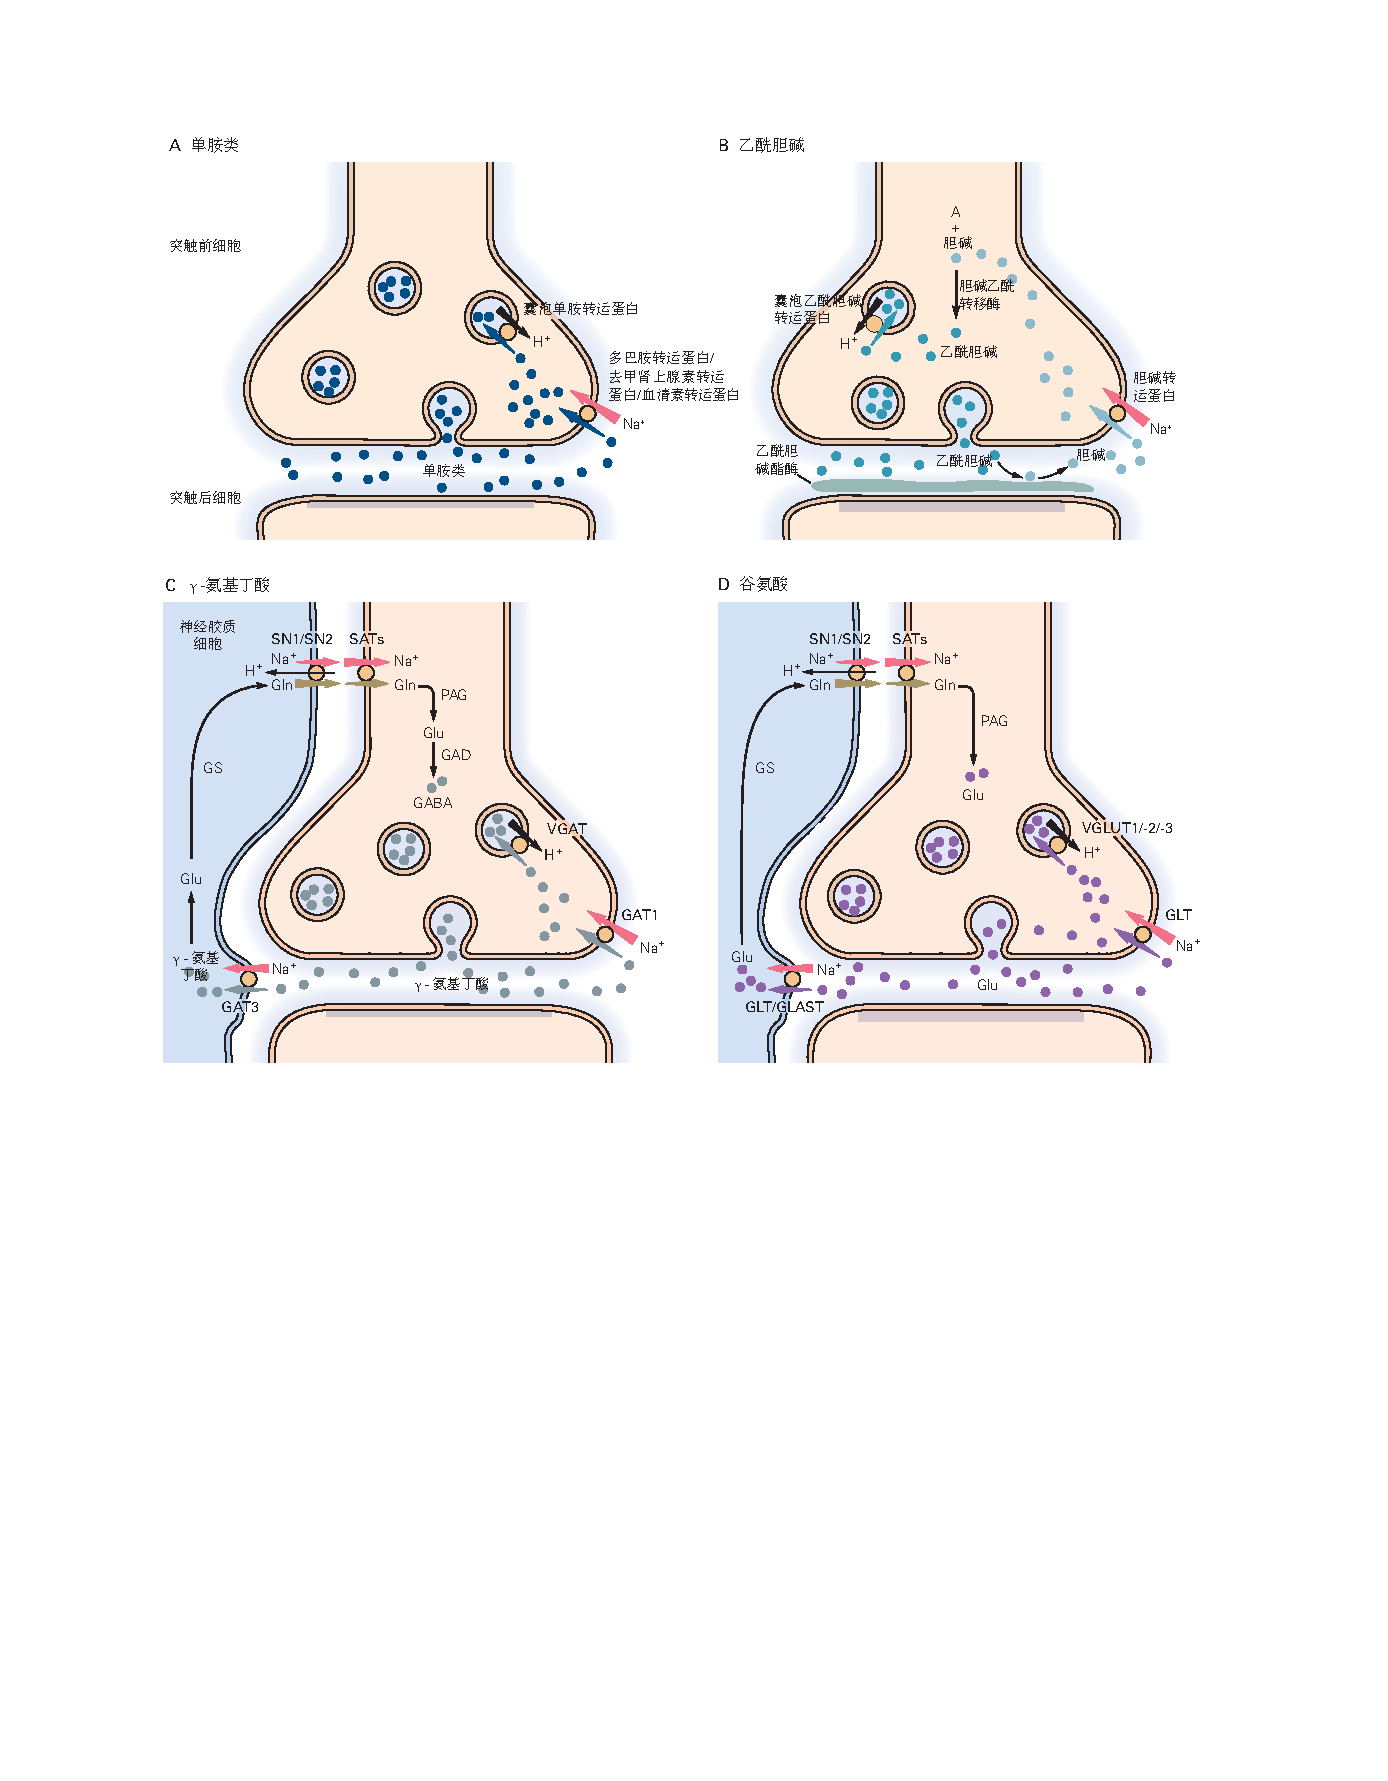
\includegraphics[width=1.0\linewidth]{chap16/fig_16_1}
	\caption{小分子递质通过转运蛋白从胞质溶胶转运到囊泡或从突触间隙转运到胞质溶胶。
		大多数小分子神经递质通过神经末梢的胞吐作用释放,并作用于特定的突触后受体。
		位于神经末梢或周围神经胶质细胞中的特定转运蛋白终止信号并回收递质。
		这些蛋白质(橙色圆圈)的运输由 \ce{H+}(黑色箭头)或 \ce{Na+}(红色箭头)的电化学梯度驱动\cite{chaudhry2008pharmacology}。
		\textbf{A.} 三种不同的转运蛋白介导单胺跨质膜的再摄取。
		\textit{多巴胺转运蛋白}、\textit{去甲肾上腺素转运蛋白}和\textit{血清素转运蛋白}负责其同源递质的再摄取(深蓝色箭头)。
		\textit{囊泡单胺转运蛋白}将所有三种单胺转运到突触小泡中,用于随后的胞吐释放。
		\textbf{B.} 胆碱能信号通过位于突触间隙(绿色条)中的\textit{乙酰胆碱酯酶}将\textit{乙酰胆碱}代谢为无活性胆碱和乙酸盐而终止。
		\textit{胆碱}由\textit{胆碱转运蛋白}转运回神经末梢(浅蓝色箭头),\textit{胆碱转运蛋白}随后催化胆碱乙酰化以重构\textit{乙酰胆碱}。
		\textit{乙酰胆碱}通过\textit{囊泡乙酰胆碱转运蛋白}转运到囊泡中。
		\textbf{C.} 在\textit{$\gamma$-氨基丁酸}能和甘氨酸能神经末梢,\textit{$\gamma$-氨基丁酸转运蛋白}和\textit{甘氨酸转运蛋白}(未显示)分别介导\textit{$\gamma$-氨基丁酸}和甘氨酸(灰色箭头)的再摄取。
		\textit{$\gamma$-氨基丁酸}也可能被周围的神经胶质细胞吸收(例如,被 GAT3)。
		在神经胶质细胞中,\textit{$\gamma$-氨基丁酸}首先通过\textit{谷氨酸脱羧酶}转化为\textit{谷氨酸}。 然后 \textit{谷氨酸}被神经胶质\textit{谷氨酰胺合成酶}转化为\textit{谷氨酰胺}。
		通过系统 N 转运蛋白(SN1/SN2)和系统 A 转运蛋白(SAT)(棕色箭头)的协同作用,谷氨酰胺被运回神经末梢。
		在神经末梢,\textit{磷酸激活的谷氨酰胺酶}将谷氨酰胺转化为谷氨酸,谷氨酸通过\textit{谷氨酸脱羧酶}转化为\textit{$\gamma$-氨基丁酸}。
		然后 VGAT 将\textit{$\gamma$-氨基丁酸}转运到囊泡中。
		神经胶质转运蛋白 GLYT1(未显示)也有助于甘氨酸的清除。
		\textbf{D.} 从兴奋性神经元末梢释放后,大部分谷氨酸被周围神经胶质细胞吸收(例如,被 GLT 和 GLAST)转化为谷氨酰胺,随后通过 SN1/SN2 和一种 SAT(SATx)(棕色箭头)。
		GLT 亚型(紫色箭头)也证明了谷氨酸能末端的谷氨酸再摄取。 谷氨酸通过 VGLUT 转运到囊泡中。}
	\label{fig:16_1}
\end{figure}


递质分子被经典地建模为被囊泡转运蛋白吸收到囊泡中,以换取将两个质子从囊泡中运出。
因为 pH 梯度的维持需要\textit{三磷酸腺苷}的水解,所以将递质摄取到囊泡中是能量依赖性的。
囊泡转运蛋白可以将一些神经递质(例如多巴胺)浓缩至相对于它们在细胞质中的浓度的 10 万倍。
转运体对递质的摄取速度很快,使囊泡在释放递质并通过内吞作用回收后能够快速重新填充;
这对于在快速神经放电期间维持可释放囊泡的供应很重要(第~\ref{chap:chap15}~章)。


底物转运蛋白的特异性变化很大。
\textit{囊泡乙酰胆碱转运蛋白}不转运胆碱或其他递质。
同样,在中枢神经系统中差异表达的三种类型(VGLUT1、2 和 3)的囊泡谷氨酸转运蛋白携带可忽略不计的其他酸性氨基酸天冬氨酸。
然而,\textit{囊泡单胺转运蛋白}可以运输所有生物胺以及药物,包括苯丙胺,甚至一些神经毒性化合物,如\textit{N-甲基-4-苯基吡啶}。
\textit{焦磷酸甲基酯}是合成阿片类滥用药物的污染物,被 B 型\textit{单胺氧化酶}代谢为\textit{N-甲基-4-苯基吡啶}。
事实上,\textit{囊泡单胺转运蛋白}1 由\textit{罗伯特$\cdot$爱德华}及其同事根据转运体保护细胞免受\textit{N-甲基-4-苯基吡啶}神经毒性作用的能力克隆;
表达\textit{囊泡单胺转运蛋白}的细胞能够将毒素隔离在囊泡样隔室中,从而降低其细胞质浓度并促进细胞存活。
通过在对\textit{N-甲基-4-苯基吡啶}敏感的哺乳动物细胞系中表达从肾上腺嗜铬细胞瘤细胞的\textit{互补脱氧核糖核酸}文库中获得的基因,\textit{爱德华}能够根据选择性存活识别表达 \textit{囊泡单胺转运蛋白}1 的细胞。
\textit{囊泡单胺转运蛋白}随后通过同源克隆以及许多其他组直接识别。


转运蛋白和 V-ATP 酶存在于小突触小泡和大致密核小泡的膜中。
囊泡转运蛋白是几种重要药理学试剂的靶标。
\textit{利血平}和\textit{丁苯那嗪}通过与囊泡单胺转运体结合来抑制胺递质的摄取。
精神兴奋剂苯丙胺、甲基苯丙胺和 3,4-亚甲二氧基-N-甲基苯丙胺(MDMA 或摇头丸)的作用是消耗胺递质分子的囊泡,但也导致它们通过质膜生物胺转运体从细胞质流出到细胞外空间,见下文)。
这些化合物通过 \textit{囊泡单胺转运蛋白} 介导的质子反向驱动运输在囊泡内积累,这减少了将胺递质加载到囊泡中所需的质子梯度。


与正常递质物质足够相似的药物可以作为假递质。
它们被包装在囊泡中并通过胞吐作用释放,就好像它们是真正的递质一样,但它们通常与天然递质的突触后受体结合很弱或根本不结合,因此它们的释放会降低传递的效率。
历史上用于治疗高血压的几种药物,如 $\alpha$-甲基多巴和胍乙啶,被吸收到肾上腺素能突触中(在 $\alpha$-甲基多巴的情况下转化为 $\alpha$-甲基多巴胺)并取代突触小泡中的去甲肾上腺素。
当释放时,这些药物不能刺激突触后肾上腺素能受体,从而通过抑制肾上腺素能张力来松弛血管平滑肌。
膳食红酒和奶酪中大量含有酪胺,它也是一种错误的递质;
但是,它也可以通过类似于苯丙胺的机制释放生物胺,从而起到兴奋剂的作用。
另一种错误递质 5-羟基多巴胺可产生电子致密反应产物,并已用于识别获取生物胺的突触小泡。


最近,设计了几种荧光假神经递质,使研究人员能够使用成像方法监测啮齿动物和苍蝇大脑突触活动期间神经递质衍生物的摄取和释放(参见方框~\ref{box:16_2}~中的图~\ref{fig:16_5})。


\begin{proposition}[神经解剖学导航术语] \label{box:16_2}
	
	\quad \quad 神经元内化学信使及其加工酶的检测
	
	\quad \quad 强大的组织化学技术可用于检测神经组织组织切片中的小分子递质和神经活性肽。
	
	\quad \quad 儿茶酚胺和5-羟色胺与甲醛蒸气反应形成荧光衍生物。
	在递质组织化学的早期例子中,瑞典神经解剖学家\textit{本特$\cdot$法尔克}和\textit{尼尔斯$\cdot$希勒}发现,该反应可用于在适当控制的条件下通过荧光显微镜定位递质。
	
	\quad \quad 由于单个囊泡太小而无法通过光学显微镜分辨,因此通过将光学显微镜下的荧光与电子显微镜下的囊泡位置进行比较,可以推断出含有发射器的囊泡的确切位置。
	许多荧光假发射器,特别是那些模拟儿茶酚胺的假发射器,是质膜和/或囊泡转运蛋白的底物,使其能够用于标记囊泡并评估其在活组织中的周转率。
	此外,基于绿色荧光蛋白的多种遗传表达的神经递质报告基因可用于检测细胞外神经递质水平。
	
	\quad \quad 组织化学分析可以扩展到特殊条件下神经元的超微结构。
	在高锰酸钾,铬酸盐或银盐或多巴胺类似物5-羟基多巴胺(形成电子致密产物)存在下固定神经组织,增强了含有生物胺的囊泡的电子密度,从而揭示了大量致密的核心囊泡,这是胺能神经元的特征。
	
	\quad \quad 还可以鉴定表达特定递质酶或肽前体基因的神经元。
	许多检测特定\textit{信使核糖核酸}的方法依赖于核酸杂交。一种这样的方法是原位杂交。
	
	\quad \quad 如果核酸聚合物的两条单链的碱基序列是互补的,则它们将配对。
	通过原位杂交,在适合与内源性(有义)\textit{信使核糖核酸}杂交的条件下,将非编码\textit{脱氧核糖核酸}链(负链或反义链或其相应的\textit{核糖核酸})应用于组织切片。
	如果探针被放射性标记,放射自显影可以揭示神经元的位置,这些神经元包含由标记的互补核酸链和\textit{信使核糖核酸}形成的复合物。
	
	\quad \quad 用含有化学标记,荧光标记或用抗体标记的碱基类似物的核苷酸合成的杂合寡核苷酸可以通过组织化学检测。
	可以同时使用多个标签(图~\ref{fig:16_3}A)。
	RNAscope是一种最新的\textit{信使核糖核酸}杂交方法,可以同时检测具有较低背景和单分子灵敏度的不同\textit{信使核糖核酸}。
	检测合成蛋白的另一种方法涉及与绿色荧光蛋白变体融合的蛋白的病毒或转基因表达(图~\ref{fig:16_3}B)。
	
	\quad \quad 还可以使用免疫组织化学技术检测递质物质。
	氨基酸递质,生物胺和神经肽具有一个伯氨基,该伯氨基在神经元内共价固定;该组通过醛与蛋白质交联,醛是免疫组织化学技术显微镜中常用的固定剂。
	
	\quad \quad 针对递质物质的特异性抗体是必要的。
	对血清素、组胺和许多神经活性肽具有特异性的抗体可以通过第二种抗体检测(在一种称为间接免疫荧光的技术中)。
	例如,如果第一抗体是兔源性的,则第二抗体可以是针对兔免疫球蛋白产生的山羊抗体。
	
	\quad \quad 这些市售的二抗用荧光染料标记,并在荧光显微镜下用于在单个神经元细胞体,轴突和突触前释放位点的区域中定位抗原(图~\ref{fig:16_3})。
	
	\quad \quad 免疫组织化学技术也与电子显微镜一起用于定位神经元超微结构中的化学递质。
	这些技术通常涉及产生电子致密反应产物的过氧化物酶-抗过氧化物酶系统。
	另一种方法是使用与电子致密金颗粒相连的抗体。
	胶体金球体可以在纳米范围内产生精确的直径。
	当用适当的抗体包被时,这些金颗粒可用于高分辨率检测蛋白质和肽。
	该技术还有一个额外的有用功能,即如果每种抗体都与不同大小的金颗粒相连,则可以在同一组织切片中检查一种以上的特异性抗体(图~\ref{fig:16_4})。
	
	\quad \quad 许多荧光囊泡转运蛋白底物已被用作\textit{荧光假神经递质},以监测小鼠大脑切片或整个苍蝇大脑中递质的释放(图~\ref{fig:16_5})。
	这种方法可以可视化突触小泡中装有\textit{荧光假神经递质}的神经末梢;
	然后可以实时光学监测释放,以响应去极化(导致胞吐和突触囊泡排空)或苯丙胺(导致囊泡内容物非细胞释放到细胞质中以响应囊泡脱酸)。
	
\end{proposition}


\begin{figure}[htbp]
	\centering
	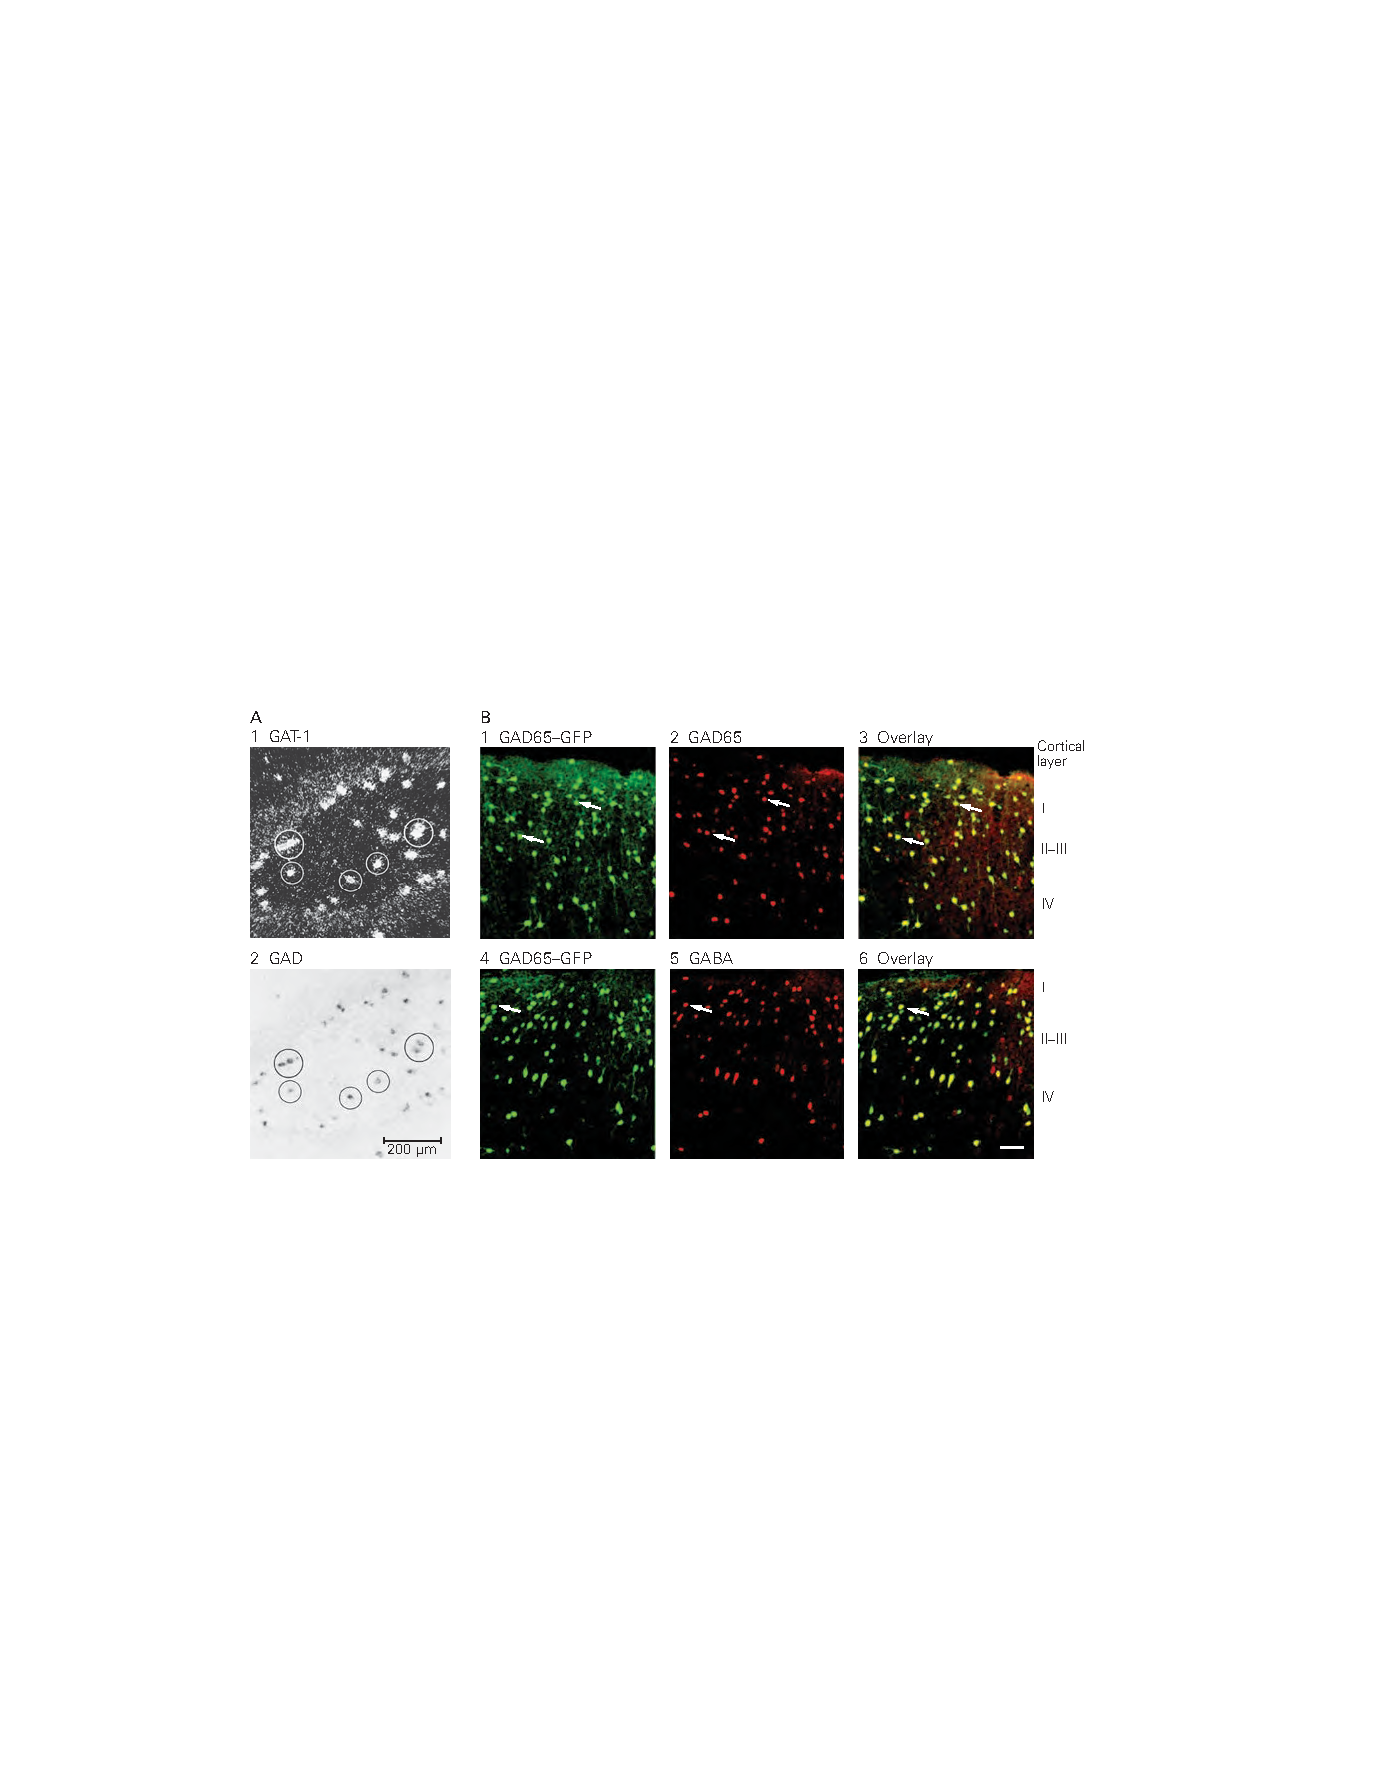
\includegraphics[width=0.85\linewidth]{chap16/fig_16_3}
	\caption{可视化化学信使的技术。
		\textbf{A.} 大鼠海马体的光学显微镜切片。
		1.使用编码\textit{$\gamma$-氨基丁酸}转运蛋白GAT-1的\textit{信使核糖核酸}的探针的原位杂交。
		用$\alpha$-35S dATP对探针进行末端标记,并通过覆盖的放射自显影照相乳剂中的银颗粒簇进行观察。
		2.用与碱性磷酸酶连接的寡核苷酸探针对\textit{谷氨酸脱羧酶}的\textit{信使核糖核酸}进行原位杂交,\textit{谷氨酸脱羧酶}是$\gamma$-氨基丁酸的特异性生物合成酶。
		\textit{谷氨酸脱羧酶}探针通过细胞质中有色碱性磷酸酶反应产物的积累而显现。
		表达GAT-1和\textit{谷氨酸脱羧酶}转录物的神经元分别用银粒和磷酸酶反应标记,并用包含这两种标记的细胞体周围的圆圈表示。
		\textbf{B.} 来自\textit{谷氨酸脱羧酶}65-GFP转基因小鼠的新皮层的图像,其中绿色荧光蛋白(GFP)在\textit{谷氨酸脱羧酶}65启动子的控制下表达。
		GFP与\textit{谷氨酸脱羧酶}65(1-3)和\textit{$\gamma$-氨基丁酸}(4-6)(均通过间接免疫荧光检测)共同定位于不同层的神经元中。
		大多数GFP阳性神经元对\textit{谷氨酸脱羧酶}65和\textit{$\gamma$-氨基丁酸}呈免疫阳性(箭头显示所选实例)。
		比例尺=100 微米。}
	\label{fig:16_3}
\end{figure}


\begin{figure}[htbp]
	\centering
	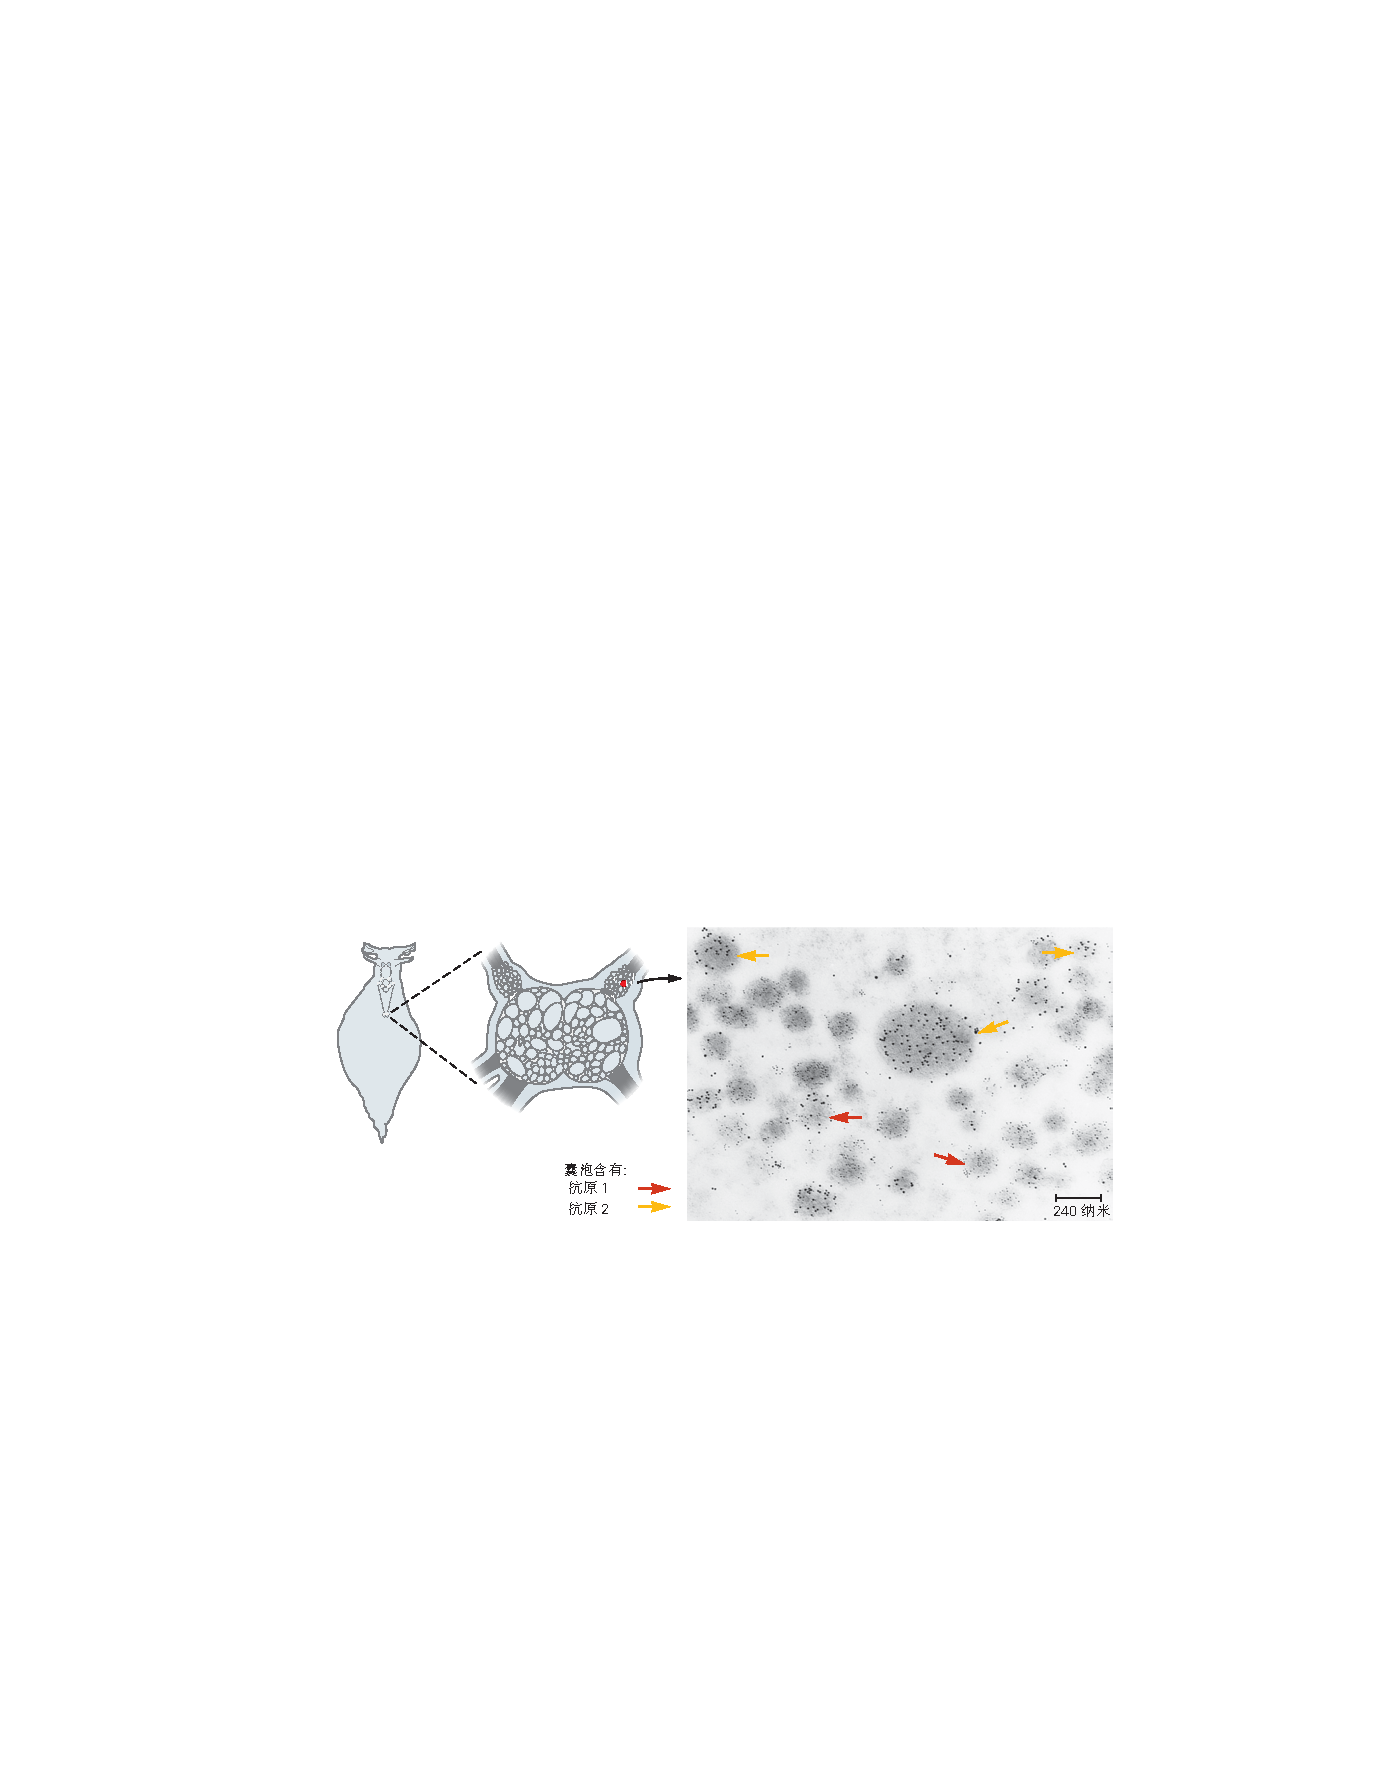
\includegraphics[width=0.9\linewidth]{chap16/fig_16_4}
	\caption{与抗体相连的电子不透明金颗粒用于在超微结构水平上定位组织中的抗原。
		电子显微照片显示了穿过海兔袋细胞的细胞体的截面。
		囊细胞通过释放一组从\textit{产卵激素}前体切割而来的神经肽来控制生殖行为。细胞含有几种致密的核心囊泡。
		用针对\textit{产卵激素}前体的不同区域中所含的不同氨基酸序列的两种抗体处理此处显示的细胞。
		一种抗体在兔子身上产生,另一种在大鼠身上产生。
		用山羊饲养的抗兔或抗大鼠免疫球蛋白(第二抗体)检测这些抗体。
		每种二级抗体都与不同大小的胶体金颗粒偶联。
		由抗原1鉴定的囊泡(用较小的金颗粒标记)小于由抗原2鉴定的囊袋(用较大的金颗粒标记),这表明从前体切割的特异性片段定位在不同的囊泡中。}
	\label{fig:16_4}
\end{figure}



\begin{figure}[htbp]
	\centering
	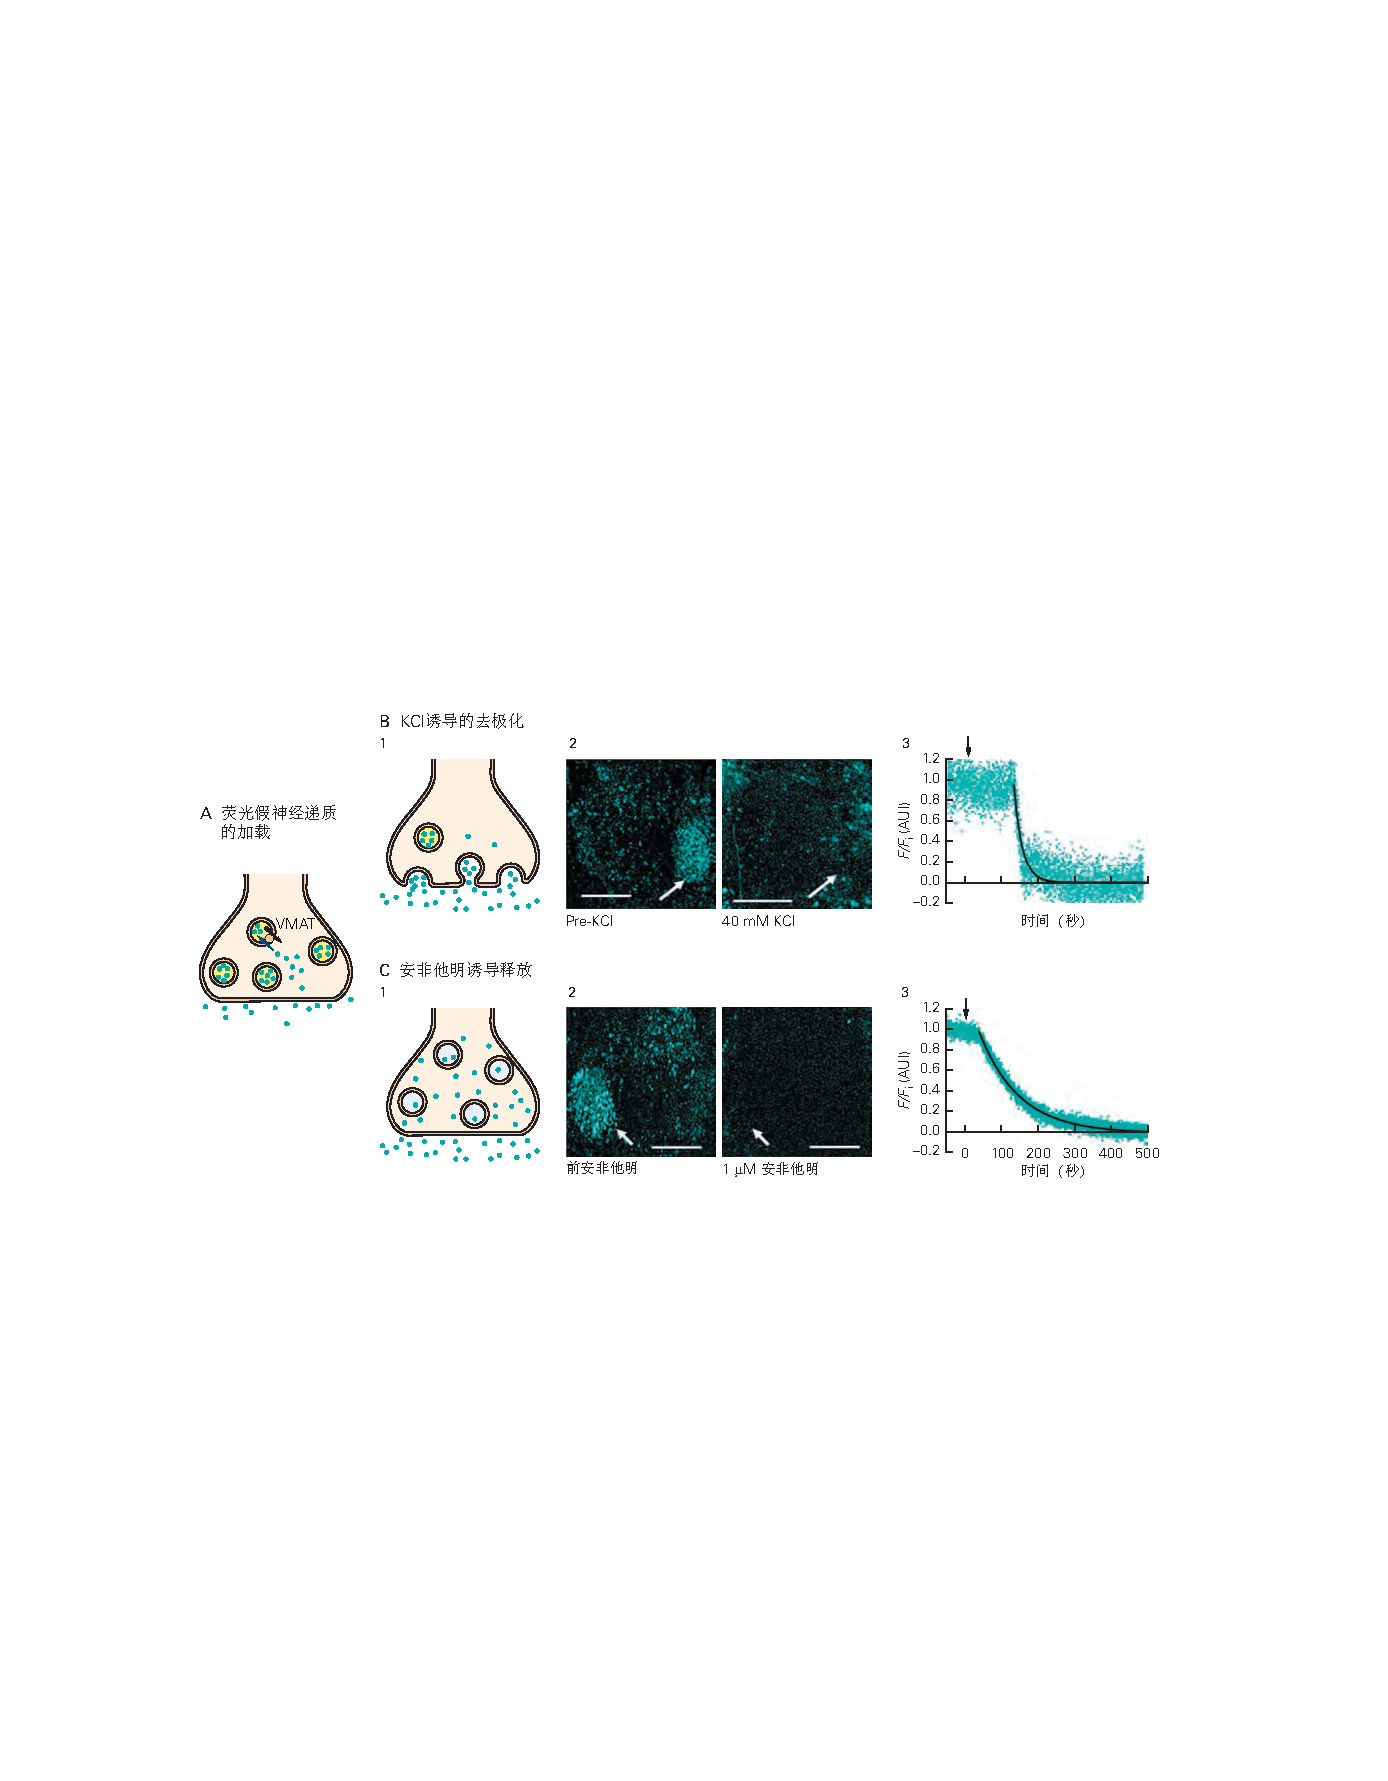
\includegraphics[width=0.9\linewidth]{chap16/fig_16_5}
	\caption{\textit{荧光假神经递质}标记允许对神经递质释放进行光学监测。
		\textbf{A.} \textit{荧光假神经递质}(蓝点)由\textit{囊泡单胺转运蛋白}转运到多巴胺神经末梢的突触小泡中。
		稳定状态下的囊泡呈酸性,如黄色阴影所示。
		\textbf{B.} 1. 提高细胞外 KCl 浓度导致去极化并通过胞吐作用释放囊泡,导致荧光标记丢失(脱色)。
		2. KCl(40 毫摩尔)去极化导致突触前多巴胺神经末梢的 \textit{荧光假神经递质}206 快速脱色。
		用 \textit{荧光假神经递质}206(300 纳摩尔)将整个果蝇大脑加载到稳定状态,并用 KCl 处理。
		在 KCl 诱导的去极化之前(左)和之后(右)神经细胞的投射图像堆栈。
		3. 代表性实验的荧光衰减动力学。
		黑色箭头表示开始添加 KCl。
		比例尺 = 25 微米。
		\textbf{C.} 1. 苯丙胺通过文中讨论的非胞吐机制导致囊泡脱酸(黄色阴影消失)及其脱色。
		2. 苯丙胺(1 微摩尔)导致 \textit{荧光假神经递质}206 脱色。
		用\textit{荧光假神经递质}206(300 纳摩尔)将整个果蝇大脑加载到稳定状态,并用苯丙胺处理。
		治疗前(左)和治疗后(右)神经细胞的投射图像堆栈。
		3. 代表性实验的荧光衰减动力学。
		黑色箭头表示开始添加药物。
		比例尺 = 25 微米。}
	\label{fig:16_5}
\end{figure}


一个意外的发现是,尽管树突中缺乏突触小泡,但多巴胺可以从树突和轴突中释放出来。
表达\textit{囊泡单胺转运蛋白}的细胞器似乎可能是释放的来源,尽管对细胞内 \ce{Ca^2+} 的要求不同于突触前末梢的经典神经传递。
由于技术原因,这种现象主要在黑质多巴胺能神经元的树突中进行了研究:多巴胺可以通过电化学技术直接测量,并且树突与细胞体很好地分离。
然而,树突状神经递质释放可能在整个神经系统中更广泛地发生。



\section{许多神经活性肽充当递质}

在细胞质中发现了催化低分子量神经递质合成的酶,多巴胺 $\beta$-羟化酶除外。
这些酶在细胞体中的游离多核糖体上合成,可能在树突中合成,并通过轴浆流分布在整个神经元中。
这样,神经元的各个部分都可以形成小分子的递质物质; 最重要的是,它们可以在释放它们的轴突突触前位点合成。


相反,神经活性肽来源于细胞体中形成的分泌蛋白。
超过 50 种短肽由神经元或神经内分泌细胞产生并发挥生理作用(表~\ref{tab:16_2})。
有些作为脑外靶标的激素(例如,血管紧张素和胃泌素)或神经内分泌分泌的产物(例如,催产素、加压素、生长抑素、黄体生成素和促甲状腺素释放激素)。
此外,许多神经肽在靠近目标神经元释放时充当神经递质,在那里它们可以引起抑制、兴奋或两者。


\begin{table}[htbp]
	\caption{神经活性哺乳动物肽} \label{tab:16_2} \centering
	\begin{tabular}{ll}
		\toprule
		类别 & 肽 \\
		\midrule
		下丘脑神经肽 & 促甲状腺素释放激素  \\
		 & 促性腺激素释放激素  \\
		 & 促皮质素释放因子  \\
		 & 生长激素-释放激素  \\
		 & 黑素细胞刺激素  \\
		 & 黑色素细胞抑制因子  \\
		 & 生长激素抑制素  \\
		 & $\beta$-内啡肽  \\
		 & 强啡肽  \\
		 & 甘丙肽  \\
		 & 神经肽 Y  \\
		 & 食欲素   \\
		 & 催产素   \\
		 & 加压素   \\
		神经垂体神经肽 & 催产素   \\
		 & 加压素   \\
		垂体肽 & 促肾上腺皮质激素   \\
		 & $\beta$-内啡肽   \\
		 & $\alpha$-黑素细胞刺激素   \\
		 & 促乳素   \\
		 & 促黄体生成素   \\
		 & 生长激素   \\
		 & 促甲状腺激素   \\
		松果体激素 & 褪黑素   \\
		基底神经节 & P 物质   \\
		 & 脑啡肽   \\
		 & 强啡肽   \\
		 & 神经肽 Y   \\
		 & 神经降压素   \\
		 & 胆囊收缩素   \\
		 & 胰高糖素样肽-1   \\
		 & 可卡因和苯丙胺调节转录物   \\
		胃肠肽 & 血管活性肠多肽   \\
		 & 胆囊收缩素   \\
		 & 胃泌素   \\
		 & P 物质   \\
		 & 神经降压素   \\
		 & 蛋氨酸脑啡肽   \\
		 & 亮氨酸脑啡肽   \\
		 & 胰岛素   \\
		 & 胰高血糖素   \\
		 & 蛙皮素   \\
		 & 胰泌素   \\
		 & 生长抑素   \\
		 & 促甲状腺素释放激素   \\
		 & 胃动素   \\
		心脏 & 心钠肽   \\
		其他 & 血管紧张素Ⅱ   \\
		 & 缓激肽   \\
		 & 降钙素   \\
		 & 降钙素基因相关肽   \\
		 & 甘丙肽   \\
		 & 瘦素蛋白   \\
		 & 睡眠肽   \\
		 & K 物质(神经激肽 A)   \\
		\bottomrule
	\end{tabular}
\end{table}


神经活性肽与调节感觉知觉和影响有关。
一些肽,包括 P 物质和脑啡肽,优先位于与疼痛感知有关的中枢神经系统区域。
其他神经肽调节对压力的复杂反应;
这些肽包括 $\gamma$-黑素细胞刺激素、\textit{促肾上腺皮质激素释放激素}、\textit{促肾上腺皮质激素}、强啡肽和 $\beta$-内啡肽。


\begin{table}[htbp]
	\caption{神经活性肽的主要家族} \label{tab:16_3} \centering
	\begin{tabular}{ll}
		\toprule
		家庭 & 肽成员 \\
		\midrule
		类鸦片 & \makecell[l]{阿片皮质素、脑啡肽、强啡肽、\\FMRF酰胺(Phe-Met-Arg-Phe酰胺)}  \\
		神经垂体密封神经肽 & 加压素、催产素、后叶激素运载蛋白  \\
		速激肽 & \makecell[l]{P 物质、南美蛙皮肽、\\肛褶蛙肽、耳腺蛙肽、章鱼降压肽、\\铃蟾肽、K 物质}  \\
		胰泌素 & \makecell[l]{分泌素、胰高血糖素、血管活性肠肽、\\胃抑制肽、生长激素释放因子、\\肽组氨酸异亮氨酸酰胺}  \\
		胰岛素 & 胰岛素、胰岛素样生长因子I和II  \\
		生长抑素 & 生长抑素,胰腺多肽  \\
		胃泌素 & 胃泌素、胆囊收缩素  \\
		\bottomrule
	\end{tabular}
\end{table}


尽管神经活性肽的多样性是巨大的,但作为一类,这些化学信使具有共同的细胞生物学。
一个惊人的普遍性是,神经活性肽被归类为具有相似氨基酸残基序列的成员家族。
至少有 10 个已被确认;
表~\ref{tab:16_3}~列出了七个主要家族。


几个不同的神经活性肽可以由一个连续的\textit{信使核糖核酸}编码,它被翻译成一个大的多蛋白前体(图~\ref{fig:16_2})。
多蛋白可以作为一种扩增机制,通过从一种前体提供超过一个拷贝的相同肽。
例如,胰高血糖素的前体含有两个拷贝的激素。
多蛋白还通过产生从一种前体裂解的几种不同的肽来产生多样性,如阿片样肽的情况。
阿片肽来源于由三个不同基因编码的多蛋白。
这些肽是 G 蛋白偶联受体家族的内源性配体。
除了内源性激动剂外,$\mu$ 阿片受体还结合具有镇痛和成瘾特性的药物,例如吗啡和合成衍生物,包括海洛因和羟考酮。


\begin{figure}[htbp]
	\centering
	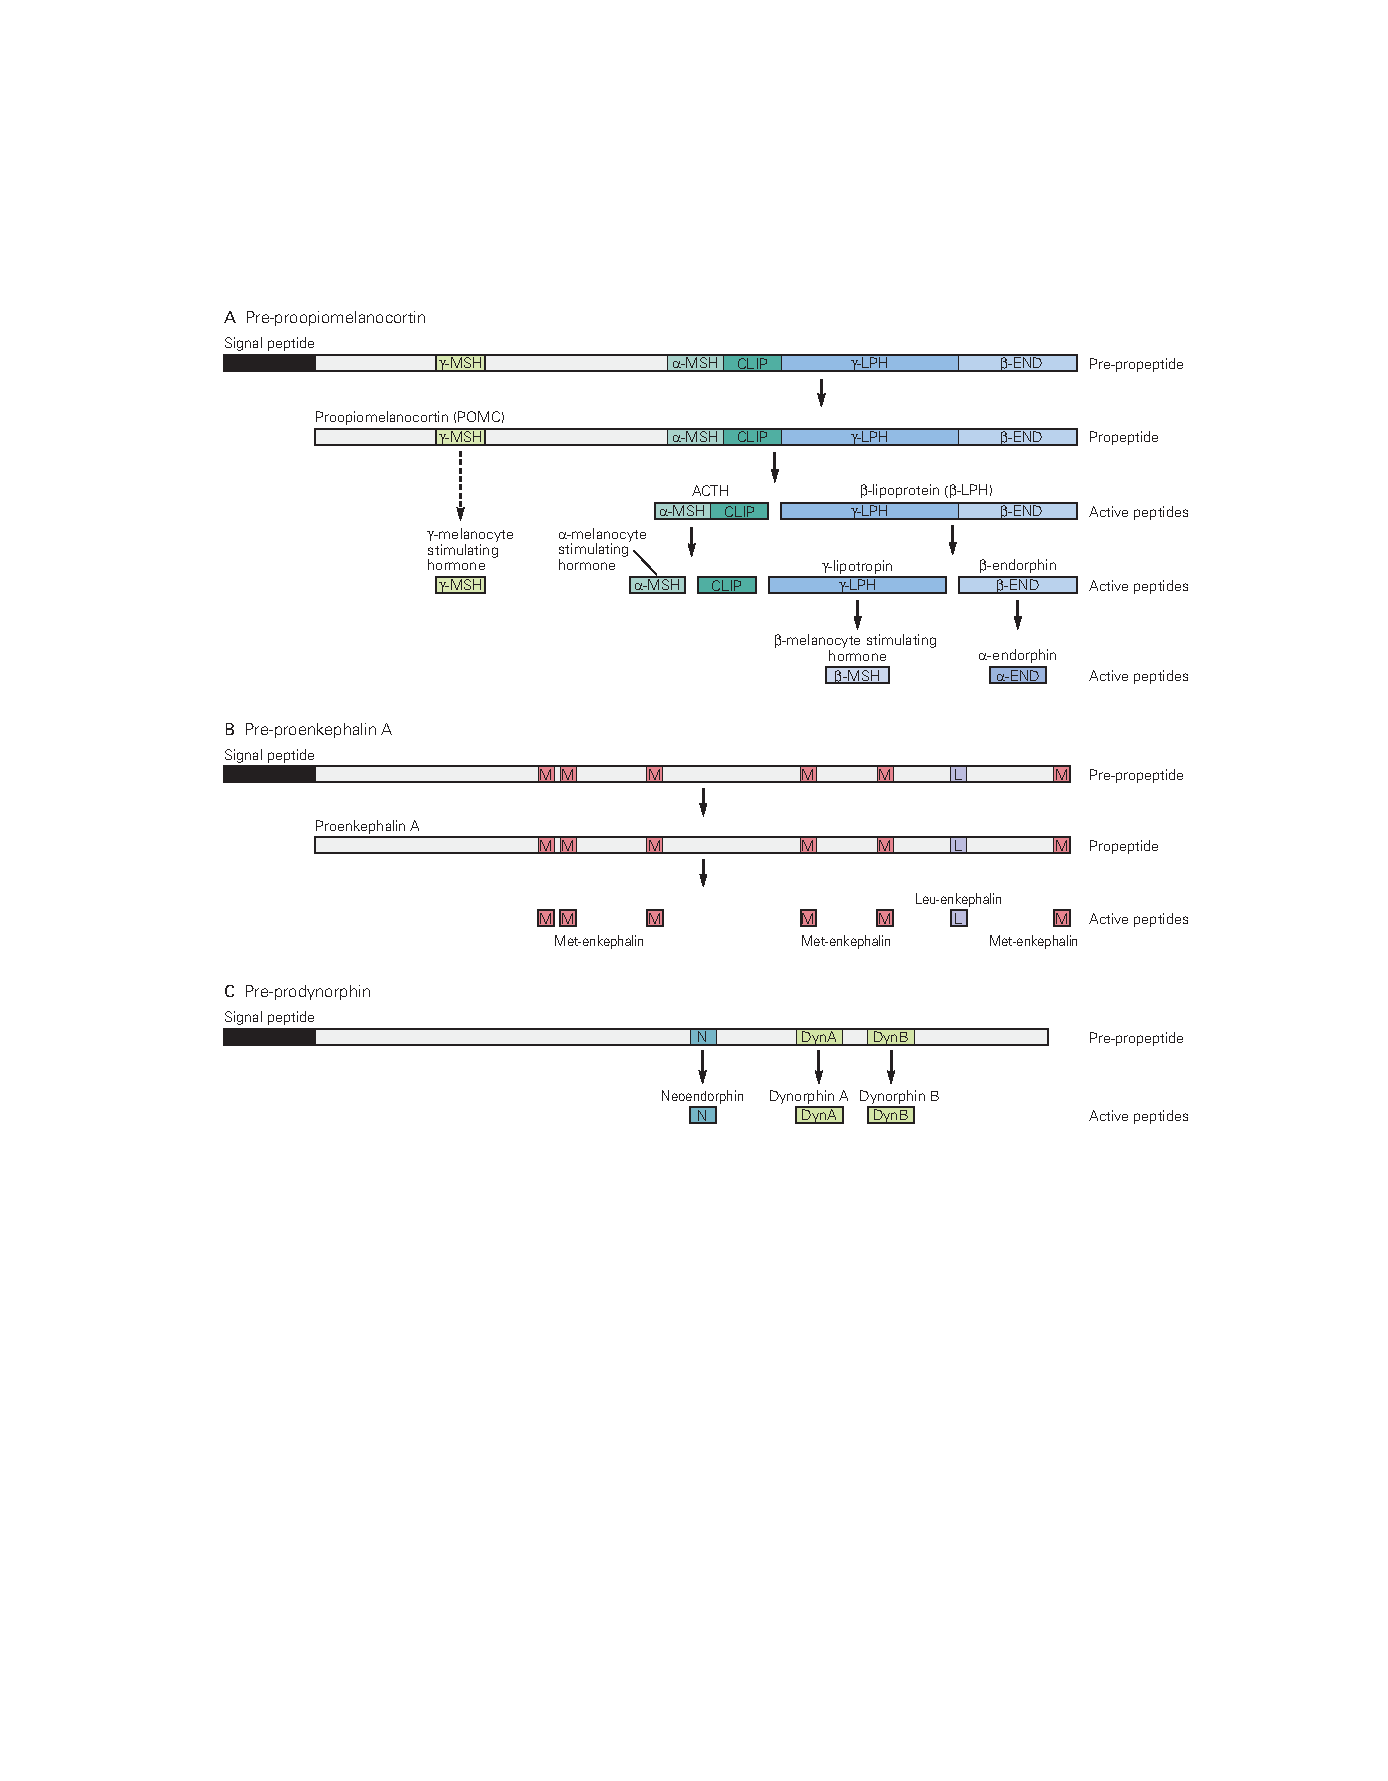
\includegraphics[width=1.0\linewidth]{chap16/fig_16_2}
	\caption{激素和神经肽前体的处理方式不同:神经肽的阿片类药物家族。
		阿片类神经肽源自较大的前体分子,需要多轮蛋白酶介导的裂解。
		这些前体经过不同的处理以产生其特定的肽产品。
		这些前体通过内质网膜的转运是由疏水信号序列启动的。
		内部切割通常发生在多肽内的碱性残基处。
		此外,这些前体具有在其加工和功能中发挥作用的关键半胱氨酸残基和糖部分。
		通常,处理的第一次迭代从新合成的多蛋白前体(称为前肽形式)开始。
		氨基末端信号序列的切割产生较小的分子,即前肽。
		三种主要的阿片肽前体蛋白由三个基因编码:\textit{前阿黑皮素}、\textit{前脑啡肽}和\textit{前强啡肽}(未显示)。
		三种合成前肽的差异加工产生了主要的阿片肽:内啡肽、脑啡肽和强啡肽。
		\textbf{A.} \textit{前阿黑皮素}前体在垂体的不同叶中以不同方式加工,产生 \textit{$\alpha$-促黑素细胞激素}和\textit{$\gamma$-黑素细胞刺激素}、\textit{促皮质激素样中间肽}和 $\beta$-促脂素。 
		\textit{$\beta$-促脂素}被裂解产生 \textit{$\gamma$-促脂素}和\textit{$\beta$-内啡肽},它们本身分别产生 $\beta$-黑素细胞刺激素(\textit{$\beta$-黑素细胞刺激素})和\textit{$\alpha$-内啡肽}。
		\textit{促肾上腺皮质激素}和\textit{$\beta$-促脂素}内的内切蛋白水解裂解发生在中叶,而不是前叶。
		\textbf{B.} 类似的原理在脑啡肽前体的加工中很明显,它产生了六种 Met-脑啡肽和一种 Leu-脑啡肽。
		\textbf{C.} 强啡肽前体被切割成至少三种与亮氨酸脑啡肽相关的肽,因为所有三种肽的氨基末端序列都含有亮氨酸脑啡肽的序列。}
	\label{fig:16_2}
\end{figure}


从单一多蛋白加工出一种以上的功能肽并不是神经活性肽所独有的。
该机制首先针对由小\textit{核糖核酸}病毒编码的蛋白质进行了描述。
几种病毒多肽是由相同的病毒多聚蛋白产生的,并且都有助于新病毒颗粒的产生。
与病毒一样,不同的蛋白质显然服务于共同的生物学目的(新病毒的形成),神经元多肽在许多情况下会产生协同工作以服务于共同的生理目标的肽。
有时生物功能似乎更复杂,因为具有相关或拮抗活性的肽可以从相同的前体产生。


这种形式的协同作用的一个特别引人注目的例子是由\textit{产卵激素}的前体形成的一组肽,这是一组控制海洋软体动物\textit{海兔}不同生殖行为的神经肽。
产卵激素可以作为引起输卵管肌肉收缩的激素;
它也可以作为一种神经递质来改变参与产生行为的几个神经元的放电,就像从多蛋白上切下的其他肽一样。


神经活性肽的加工过程发生在神经元的细胞内膜系统和囊泡中。
在这些内部膜系统内的蛋白酶的催化下,通过有限和特定的蛋白水解裂解,从单一多蛋白产生几种肽。
其中一些酶是丝氨酸蛋白酶,这一类还包括胰酶胰蛋白酶和胰凝乳蛋白酶。
与胰蛋白酶一样,肽键的切割位点由底物蛋白中的碱性氨基酸残基(赖氨酸和精氨酸)决定。
虽然切割最常见于双碱基残基,但它也可以发生在单个碱性残基上,多蛋白有时会在其他肽键处被切割。


其他类型的肽酶也催化加工神经活性肽所需的有限蛋白水解。
其中包括硫醇内肽酶(具有类似于胃蛋白酶的催化机制)、氨基肽酶(去除肽的 N 末端氨基酸)和羧肽酶 B(一种从 C 末端去除氨基酸的酶 如果肽是碱性的)。


由于处理多蛋白的方式不同,产生相同多蛋白的不同神经元可能会释放不同的神经肽。
一个例子是\textit{前阿黑皮素},它是阿片类药物家族的三个分支之一。
\textit{前阿黑皮素}存在于垂体前叶和中叶、下丘脑、大脑的其他几个区域以及胎盘和肠道的神经元中。
在所有这些组织中都发现了相同的\textit{前阿黑皮素} \textit{信使核糖核酸},但不同组织中的\textit{前阿黑皮素}以受控方式产生了不同的肽。
一种可能性是,处理相同多蛋白的两个神经元可能在内质网、高尔基体或囊泡的腔内不同地表达具有不同特异性的蛋白酶。
或者,这两个神经元可能包含相同的加工蛋白酶,但每个细胞可能在不同位点糖基化共同的多蛋白,从而保护多肽的不同区域免于切割。



\section{肽和小分子递质在几个方面有所不同}

大的致密核心囊泡与非神经元细胞的分泌颗粒同源。
这些囊泡是在跨高尔基体网络中形成的,在那里它们装载有神经肽和其他蛋白质,可以形成致密核心。
然后,致密核小泡从胞体运输到轴突的突触前位点。
除了含有神经肽外,这些囊泡由于表达囊泡转运蛋白而通常含有小分子递质。
在大的致密核心囊泡通过胞吐作用释放其内容物后,膜不会再循环形成新的大的致密核心囊泡。
相反,囊泡必须通过来自体细胞的运输来替换。
相反,成熟的小突触囊泡不在体细胞中合成。
相反,它们的蛋白质成分通过大的致密核心前体囊泡的运输被递送到释放位点。
要形成成熟的小突触囊泡,前体囊泡必须首先与质膜融合。
内吞作用之后,成熟的突触小泡然后通过局部加工产生。 
一旦它们的内容物通过胞吐作用释放出来,突触小泡就可以快速回收,以在持续的神经放电期间维持它们的局部浓度。


尽管两种类型的囊泡都含有许多相似的蛋白质,但致密核心囊泡缺乏在活性区释放所需的几种蛋白质。
来自致密核囊泡的膜仅使用一次; 必须在细胞体中合成新的致密核心囊泡,并通过顺行运输将其运输到轴突末端。
此外,神经肽不存在摄取机制。
因此,一旦肽被释放,新的供应必须从细胞体到达。
尽管有证据表明某些轴突中存在局部蛋白质合成,但尚未证明这会提供新的肽以供释放。


大的致密核囊泡通过不专用于神经细胞且不需要活性区的胞吐机制释放其内容物;
因此,释放可以发生在具有适当融合机制的轴突膜上的任何地方。
与调节分泌的其他例子一样,致密核心囊泡的胞吐作用取决于细胞内 \ce{Ca^2+} 通过电压门控 \ce{Ca^2+} 通道的普遍升高,这些通道未定位于释放位点。
因此,这种形式的胞吐作用很慢,需要高刺激频率才能将 \ce{Ca^2+} 升高到足以触发释放的水平。
这与单个动作电位后突触小泡的快速胞吐形成对比,后者通过紧密聚集在活性区的电压门控 \ce{Ca^2+} 通道启动大量、快速的 \ce{Ca^2+} 增加(第~\ref{chap:chap15}~章)。



\section{肽和小分子递质可以共同发布}

神经活性肽、小分子递质和其他神经活性分子共存于某些神经元的同一个致密核心囊泡中(第~\ref{chap:chap7}~章和第~\ref{chap:chap15} ~章)。
在成熟的神经元中,这种组合通常由一种小分子递质和一种或多种源自多蛋白的肽组成。
例如,\textit{乙酰胆碱}和\textit{血管活性肠肽}可以一起释放并协同作用于相同的靶细胞。


另一个例子是\textit{降钙素基因相关肽},它在大多数脊髓运动神经元中与\textit{乙酰胆碱}一起包装,\textit{乙酰胆碱}是神经肌肉接头处使用的递质。
\textit{降钙素基因相关肽}激活腺苷酸环化酶,提高目标肌肉中的\textit{环磷酸腺苷}水平和\textit{环磷酸腺苷}依赖性蛋白磷酸化(第~\ref{chap:chap14}~章)。
增加的蛋白质磷酸化导致收缩力增加。
另一个例子是海马体神经元中谷氨酸和强啡肽的共同释放,其中谷氨酸是兴奋性的而强啡肽是抑制性的。
因为突触后靶细胞具有两种化学信使的受体,所以所有这些共同释放的例子也是共同传递的例子。


如前所述,释放肽的致密核心囊泡不同于仅释放小分子递质的小透明囊泡。
含肽的囊泡可能含有也可能不含小分子递质,但这两种类型的囊泡都含有\textit{三磷酸腺苷}。
结果,\textit{三磷酸腺苷}通过大的致密核心小泡和突触小泡的胞吐作用释放。
此外,似乎\textit{三磷酸腺苷}可能以多种不同的方式存储和释放:
(1)\textit{三磷酸腺苷}与递质共同储存和共同释放,
(2)\textit{三磷酸腺苷}释放是同时的但独立于递质释放,以及 
(3)\textit{三磷酸腺苷}是单独释放。
\textit{三磷酸腺苷}的共同释放(释放后可降解为腺苷)可能是共存和共同释放并不一定意味着共同传递的重要说明。
\textit{三磷酸腺苷}和许多其他物质一样,可以从神经元中释放出来,但如果附近没有受体,它仍然不会参与信号传递。


如前所述,判断某种物质是否用作递质的一个标准是该物质在神经元中的浓度很高。
识别特定神经元中的递质对于理解突触传递很重要,并且使用多种组织化学方法来检测神经元中的化学信使(方框~\ref{box:16_2})。


谷氨酸突触小泡转运蛋白 VGLUT2 和 VGLUT3 在释放其他类别神经递质的神经元中表达,特别是胆碱能神经元、血清素能神经元和儿茶酚胺能神经元。
两个小分子递质共同释放的一个有趣例子是投射到腹侧纹状体、皮层和其他地方的神经元释放谷氨酸和多巴胺。
这种共同释放可能对动机行为的调节和轴突投射模式的建立具有重要意义。
在某些情况下,谷氨酸与多巴胺一起释放,以响应多巴胺能神经元放电的不同模式。
虽然关于相同的突触小泡是否可以积累两种神经递质存在争议,但在孤立的突触小泡中,谷氨酸摄取通过增加驱动小泡单胺运输的 pH 梯度来增强小泡单胺储存,提供调节量子大小的突触前机制。



\section{从突触间隙移除递质终止突触传递}

及时从突触间隙中移除递质对突触传递至关重要。
如果允许在一个突触动作中释放的递质分子在释放后保留在裂隙中,这将阻碍信号的正常空间和时间动态,最初增强信号但阻止新信号通过。
突触最终会变得难治,主要是因为持续暴露于递质导致受体脱敏。


递质物质通过三种机制从裂缝中移除:
扩散、酶促降解和再摄取。
扩散去除了所有化学信使的一部分,但在神经支配非常高的大脑区域,因此对神经递质释放有很高的要求,扩散在逐渐变细的信号传导中可以发挥相对较小的作用。
相反,在低神经支配区域,扩散是信号减少的主要方式。


在胆碱能突触中,清除\textit{乙酰胆碱}的主要方式是乙酰胆碱酯酶对递质的酶促降解。
在神经肌肉接头处,突触前神经末梢的活动区恰好位于肌肉膜的连接褶皱上方。
\textit{乙酰胆碱}受体位于面向释放位点的肌肉表面,不会深入褶皱(见图~\ref{fig:12_1}),而乙酰胆碱酯酶固定在褶皱内的基底膜上。
递质、受体和降解酶的这种解剖结构有两个功能。


首先,在释放时,\textit{乙酰胆碱}与其受体发生反应;
从受体解离后,\textit{乙酰胆碱}扩散到裂隙中,并被乙酰胆碱酯酶水解为胆碱和乙酸。
结果,递质分子仅被使用一次。
因此,酯酶的一个功能是打断突触信息。
其次,重新捕获可能因从突触间隙扩散而丢失的胆碱。
一旦被酯酶水解,胆碱就会停留在由连接褶皱提供的储库中,并被高亲和力的胆碱转运体带回胆碱能神经末梢。
(与生物胺不同,\textit{乙酰胆碱}本身在质膜上没有摄取机制。)除了乙酰胆碱酯酶外,\textit{乙酰胆碱}还可以被另一种酯酶丁酰胆碱酯酶降解,该酶还可以降解其他分子,包括可卡因和麻痹药物琥珀酰胆碱。
然而,丁酰胆碱酯酶的确切功能尚不完全清楚。


许多其他降解释放的递质的酶途径并不直接参与终止突触传递,但对于控制神经元内递质的浓度或使从突触间隙扩散的递质分子失活很重要。
许多这些降解酶在临床上很重要,它们为药物作用提供位点并用作诊断指标。
例如,\textit{单胺氧化酶}抑制剂是一种降解胺递质的细胞内酶,可用于治疗抑郁症和帕金森病。
\textit{儿茶酚氧位甲基转移酶}是另一种对降解生物胺很重要的细胞质酶。
其代谢物的测量提供了影响神经组织中生物胺合成或降解的药物功效的有用临床指标。
由于多巴胺摄取转运蛋白水平较低,\textit{儿茶酚氧位甲基转移酶}被认为在调节皮层多巴胺水平方面发挥着特别重要的作用。
\textit{儿茶酚氧位甲基转移酶}基因中的功能多态性与认知表现相关的发现强调了这种酶的相关性。


神经肽通过细胞外肽酶的缓慢扩散和蛋白水解相对缓慢地从突触间隙中去除。
相比之下,小分子递质从突触间隙和突触外空间移除得更快。
大多数小分子神经递质失活的关键机制是质膜的再摄取。 
该机制具有双重目的,即终止递质的突触作用以及重新捕获递质分子以供后续重复使用。
尽管\textit{艾略特}在 1914 年就假设可能存在摄取转运蛋白,但他们的发现一直等到 1958 年,当时\textit{芭芭拉$\cdot$休斯}和\textit{本杰明$\cdot$布罗迪}发现血小板积累了去甲肾上腺素和血清素,它们可以相互竞争摄取。
\textit{朱利叶斯$\cdot$阿克塞尔罗德}也是\textit{布罗迪}小组的成员,不久之后使用放射性标记的底物描述了去甲肾上腺素摄取到神经元中的特征。


高亲和力摄取由神经末梢和神经胶质细胞膜中的转运蛋白分子介导。
与在反向转运机制中由 \ce{H+} 电化学梯度驱动的囊泡转运蛋白不同,质膜转运蛋白通过同向转运机制由 \ce{Na+} 电化学梯度驱动,其中 \ce{Na+} 离子和递质在同一方向移动。


每种类型的神经元都有其特有的摄取机制。
例如,非胆碱能神经元不会以高亲和力摄取胆碱。
某些强效精神药物可以阻断摄取过程。
例如,可卡因会阻碍多巴胺、去甲肾上腺素和血清素的摄取;
三环类抗抑郁药会阻断血清素和去甲肾上腺素的摄取。
选择性 5-羟色胺再摄取抑制剂,如\textit{百忧解},是一项重要的治疗创新,通常比三环类抗抑郁药具有更好的耐受性,尽管难治性抑郁症仍然是一个关键问题。
应用适当的阻断转运蛋白的药物可以延长和增强生物胺和\textit{$\gamma$-氨基丁酸}的突触信号。
在某些情况下,药物既作用于神经元表面的转运蛋白,也作用于细胞内的囊泡转运蛋白。
例如,神经元外膜上的多巴胺或其他生物胺转运蛋白以及\textit{囊泡单胺转运蛋白}会主动摄取苯丙胺。


神经递质的转运分子属于结构和机制不同的两个不同的组。
来自这些家族中每一个的细菌同源物的高分辨率结构已经得到解决,这极大地促进了我们对转运蛋白机制的理解。


一组转运蛋白是\textit{神经递质钠转运体},这是一个跨膜蛋白超家族,可穿过质膜 12 次(对于许多原核生物同系物而言为 11 次)。
这些蛋白质由假对称反向重复序列组成,其中跨膜片段 1 至 5 与跨膜片段 6 至 10 同源。
\textit{神经递质钠转运体}家族包括\textit{$\gamma$-氨基丁酸}、甘氨酸、去甲肾上腺素、多巴胺、血清素、渗透素和氨基酸的转运蛋白。
人类血清素转运蛋白和苍蝇多巴胺转运蛋白的晶体结构与先前结晶的细菌同系物具有相同的结构和一般机制,最近已得到解决。


第二个家族由谷氨酸转运蛋白组成。
这些蛋白质八次穿过质膜并包含两个螺旋发夹,它们被认为在底物从膜的每一侧进入门控中起作用(见图~\ref{fig:8_16})。
每组包括针对每种递质物质的几种转运蛋白;
例如,有多种\textit{$\gamma$-氨基丁酸}、甘氨酸和谷氨酸转运蛋白,每一种都有不同的定位、功能和药理学。


可以在功能上区分这两个组。
尽管两者均由 \ce{Na+} 梯度提供的电化学势驱动,但谷氨酸的转运需要 \ce{K+} 的反向转运,而\textit{神经递质钠转运体}蛋白的转运通常需要 \ce{Cl-} 的共转运(或原核同源物中的 \ce{H+} 反向转运)。
在谷氨酸转运过程中,递质的一个带负电荷的分子与三个 \ce{Na+} 离子和一个质子(同步输运)一起输入,以换取一个 \ce{K+} 的输出。
这导致每个传输周期净流入两个正电荷,从而产生内向电流。
这种电荷转移的结果是,细胞的负静息电位产生了巨大的内向驱动力,导致细胞膜上出现巨大的谷氨酸梯度。
相反,\textit{神经递质钠转运体}蛋白与其底物一起运输一到三个 \ce{Na+} 离子和一个 \ce{Cl-} 离子。
虽然在大多数情况下,电化学驱动力足以使\textit{神经递质钠转运体}转运蛋白携带递质进入细胞,从而增加细胞质递质浓度,但细胞质中递质的浓度很低,最终由囊泡转运蛋白将递质加载到细胞中的作用决定 突触小泡。


\textit{神经递质钠转运体}蛋白功能的一个迷人方面是这些转运蛋白向后运行的能力,使它们能够产生递质流出。
这是神经递质多巴胺的最佳特征,因为苯丙胺和相关类似物通过非胞吐机制导致多巴胺大量释放。
如前所述,在药理学剂量下,苯丙胺通过质膜\textit{多巴胺转运蛋白}和囊泡\textit{囊泡单胺转运蛋白}主动转运;
后一种效应消散了囊泡 \ce{H+} 梯度,导致多巴胺逃逸到细胞质中。
然后,这种多巴胺通过\textit{多巴胺转运蛋白}“向后”移出细胞,这一过程需要对其 N 末端进行磷酸化。
虽然对于安非他明的功能至关重要,但这种磷酸化的正常生理作用仍然是个谜,因为它似乎对多巴胺摄取不是必需的。
计算研究表明,磷酸化调节的 N 末端与内叶中酸性脂质的相互作用在调节转运蛋白功能中发挥作用。
然而,最终的答案可能需要包括 N 端域的原子分辨率结构以及 N 端动力学的生物物理数据。



\section{亮点}

1. 神经元携带的信息被编码为电信号,电信号沿着它的轴突传播到突触,在那里这些信号被一个或多个化学信使转换并穿过突触间隙。


2. 两大类化学信使,小分子递质和神经活性肽,被包装在突触前神经元内的囊泡中。
在细胞质中合成后,小分子递质被吸收并高度集中在囊泡中,在那里它们免受细胞质中的降解酶的影响。


3. 周围的突触小泡高度集中在神经末梢,而在大脑中,往往在突触前部位沿轴突静脉曲张。
具有离子型谷氨酸受体的经典兴奋性突触是与紧密并列的突触后结构(例如树突棘)通信的“私有”突触的示例。
相比之下,多巴胺系统举例说明了可以与许多神经元上的突触外受体相互作用的“社交”突触。


4. 为了防止快速突触传递过程中小分子递质的耗尽,大多数是在末端局部合成的。


5. 神经活性肽的蛋白质前体仅在细胞体内合成,即转录和翻译的部位。
神经肽被包装在分泌颗粒和囊泡中,通过轴浆运输从细胞体运送到末端。
与包含小分子递质的囊泡不同,这些囊泡不会在末端重新填充。 


6. 调节递质生物合成的酶受到严格的调控,神经元活动的变化会导致这些酶的水平和活性发生稳态变化。
由于磷酸化和去磷酸化反应,以及通过细胞核中的转录控制,这种调节可以发生在细胞质中的翻译后。 


7. 终止发射器动作的精确机制是突触传输中的一个关键步骤,它几乎与发射器合成和释放一样重要。
一些释放的递质由于简单地从突触间隙扩散而丢失。
然而,在大多数情况下,递质作用会被特定的分子反应终止。 


8. 乙酰胆碱被乙酰胆碱酯酶迅速水解为胆碱和乙酸。
谷氨酸、\textit{$\gamma$-氨基丁酸}、甘氨酸和生物胺被质膜上由 \ce{Na+} 梯度驱动的特定转运蛋白吸收到突触前末端和/或神经胶质细胞中。 


9. 一些最有效的精神活性化合物作用于神经递质转运体。
可卡因的精神刺激作用源于其阻止多巴胺再摄取的作用,从而增加其细胞外水平。
相反,苯丙胺及其衍生物通过涉及质膜\textit{多巴胺转运蛋白}和囊泡转运蛋白\textit{囊泡单胺转运蛋白}的机制促进多巴胺的非胞吐释放。 


10. 了解化学传递分子策略的第一步通常涉及识别突触小泡的内容。
除了那些由转运分子或通过膜扩散释放递质的情况(在气体和脂质代谢物的情况下,见第~\ref{chap:chap14}~章),只有适当包装在囊泡中的分子才能从神经元的末梢释放。
然而,并非神经元释放的所有分子都是化学信使,只有那些与适当的受体结合并在目标神经元中启动功能变化的分子才可以被有效地视为神经递质。 


11. 当递质分子与另一个细胞膜中的受体蛋白结合时,信息被传递,导致它们改变构象,导致配体门控离子通道的离子电导增加或下游信号通路的改变 G 蛋白偶联受体。 


12. 几种神经活性物质共同释放到适当的突触后受体上,允许在单个突触动作中传递大量不同的信息。


